\documentclass[10pt]{article}
\usepackage{../../local}
\urlstyle{same}

\newcommand{\classcode}{CS 189}
\newcommand{\classname}{Introduction to Machine Learning}
\renewcommand{\maketitle}{%
\hrule height4pt
\large{Eric Du \hfill \classcode}
\newline
\large{Course Notes} \Large{\hfill \classname \hfill} \large{\today}
\hrule height4pt \vskip .7em
\small{Header styling inspired by CS 70: \url{https://www.eecs70.org/}}
\normalsize
}
\linespread{1.1}
\newtheorem{theorem}{Theorem}
\begin{document}
	\maketitle
	
	\section{Introduction}

\subsection{Examples of Machine Learning}
\begin{itemize}
	\item The things listed here are just here to provide a sense of what machine learning can
		be useful for. It's not a complete list (obviously), and we will spend time
		throughout the semester learning about some of these things. 
		\begin{enumerate}[label=\roman*.]
			\item Recognizing digits in images -- this is something that people have spent a
				lot of time trying to fine tune historically. Nowadays we have it figured
				out, but it took a surprising amount of time to get this right. 
			\item Identifying a tumor in an x-ray
			\item Classifying email as spam
			\item Diagnosing a disease from symptoms
			\item Predicting the price of a stock 6 months into the future. 
			\item Predicting the 3D structure of all atoms in a protein from it's amino acid
				structure. 
		\end{enumerate}
		There are also many types of learning problems in machine learning: 
		\begin{itemize}
			\item \textit{Classification Problems}: where the output is a label from a finite
				set. 
			\item \textit{Regression Problems}: the output is real-valued 
			\item \textit{Ranking Problems}: the output only ranks examples relative
				to one another.
			\item \textit{Unsupervised Problems}: models like Chat-GPT, are used for
				generative problems. 
		\end{itemize}
\end{itemize}
\subsection{MNIST}
\begin{itemize}
	\item This is a training set of 60,000+ examples, which was a very popular dataset to grade
		ML model performance. Each digit is a 28x28 pixel of a grey level image, and the goal
		is to have a machine identify what each number is. 
	\item In essence, you can think of each
		input as a matrix with a real valued number in it.
	\item Nowadays, we've managed to get
		the error rate down to somewhere around 0.5\%. 

\end{itemize}

\subsection{Machine Learning Approach}
\begin{itemize}
	\item Essentially, the thing we are training is what's called "feature vectors", which
		train a classifier, done in what's called "training time". 
	\item At training time, the classifier then takes in new data on an untrained 
		dataset,
		and classifies them (test time). This test dataset is usually a dataset 
		in which we
		know the correct answer, which helps us evaluate how well the model behaves. 
	\item Finally, we deploy this model for its intended use. Shockingly, 
		this is the one that's easiest to forget. 
	\item In the case of training images, we turn the 2x2 matrix of image intensities 
		into a vector instead, and classify the vector 
		(this is the same process as before, no data
		is being destroyed here). 

	\item Suppose we're training a model, and our dataset looks like:

		\begin{center}
			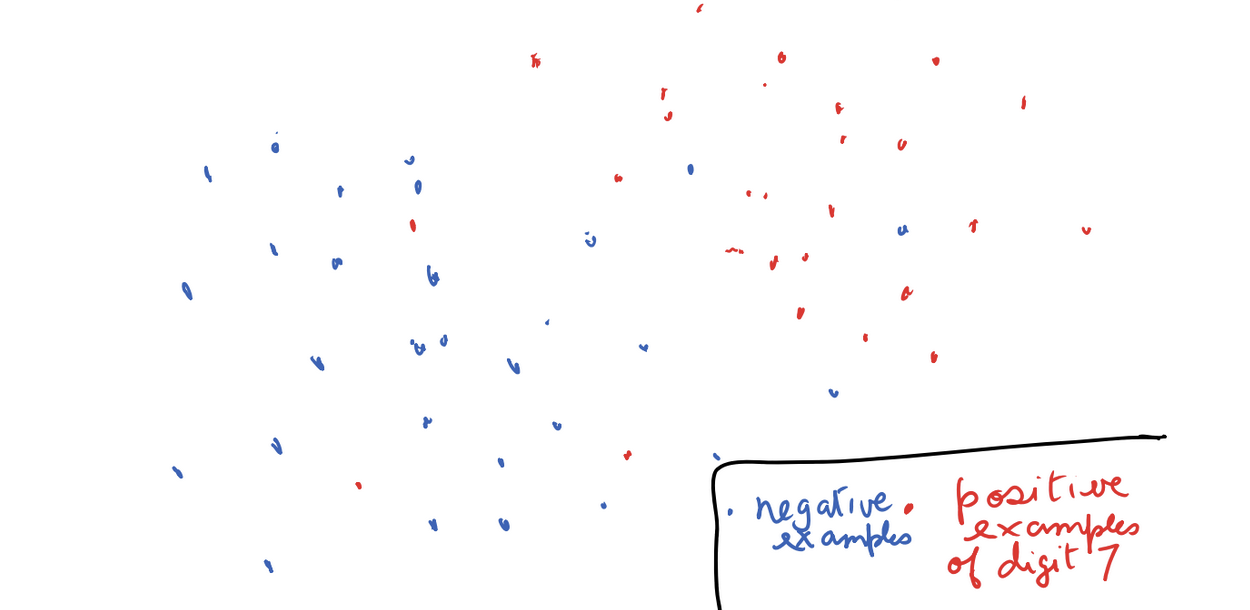
\includegraphics[scale=0.4]{lec-1a.png}
		\end{center}

		Let's say that the red dots are "positive" examples of the digit 7, and the 
		blue dots represent "negative examples" (not a 7). 
		Now, if we get a new point, how do
		we classify it?
	\item One way we can do this is via \textit{nearest neighbors}, which basically
		finds the point closest to the new data point, and classifies it as such. The
		idea here is that the similarity between the new point is highest with its
		nearest neighbor, so the probability it classifies in the same way is also
		the highest.
	\item There is also the idea of a linear classifier, where we draw a line \(
		\tilde w \cdot \tilde x + b = 0 \), which gives us a way to classify new
		point based on where they fall relative to that boundary.   
	\item Sometimes, linear classifiers aren't good enough. If our distribution is
		less skewed, then sometimes a single line isn't very effective. Sometimes, we
		can even have multiple boundaries, making the entire thing highly nonlinear.   
\end{itemize}
\subsubsection{Small aside on training error} 
\begin{itemize}
	\item Is it good to have zero training error? Yes, but only if you have a LOT of
		data. Companies like Google, Microsoft. etc. work with incredibly large
		datasets, in which case for them zero training error is a target, but if
		we're working with a smaller dataset (which will be the case at most
		companies except the largest ones), having some training error may actually
		be a good thing. 
	\item Having zero training error means that the model has basically memorized the
		training data, so there's absolutely no way that this model can be good
		elsewhere. \question{why is this?}    
\end{itemize}

\subsection{How to make nonlinear decision boundaries?}
\begin{itemize}
	\item Nearest neighbors gives us a nonlinear decision boundary, and it gets
		pretty good once we start considering multiple neighbors. 
	\item One other way we can do this is to use Neural networks to basically make
		better feature vectors directly from the initial ones. At the end, it
		generates a linear decision boundary. This is called the "latent
		representation". Then, we can build a classifier on top
		of this decision boundary. In essence, this is what a linear classifier does. 
	\item Suppose all the positive examples lie inside a disk. Then, there's no
		possible way for a linear classifier to work well on the initial data, but
		the hope is that we can use machine learning to generate another feature
		space where a linear classifier \textit{would} work.    

		For the disk example, we could take a boundary \( x_1^2 + x_2^2 = c \), then
		the classification is linear with respect to \( x_1^2 \) and \( x_2^2 \)!
		Therefore, we can perform a linear classification here. In our case, our
		features could be:
		\[
			\begin{bmatrix} x_1 \\ x_2 \\ x_1^2 \\ x_1x_2 \\ x_2^2 \end{bmatrix}
		\]
		Note that this doesn't change our data at all, it just modifies it in a way
		so that we can perform linear regression on it. Here, we would try to find
		a linear classifier in this 5-dimensional space.       
\end{itemize}

\subsection{Neural Networks}
\begin{itemize}
	\item All they are is just composing simple logistic regression functions over
		and over again.  
	\item For a single layer, single output neural network, it would take each input,
		and have its own weight \( w_i \) associated with them. Then, we can output
		something along the lines of:
		\[
			v_2 = \sum_k w_{k}x_k 
		\]
		In other words, we can think of this as an inner product between our input
		and the weight vector.   
	\item Then, what we will do is to introduce some nonlinearity into the equation,
		so that we can get something meaningful out of the neural network. If we just
		keep repeating this with linear functions, then we're obviously going to get
		something linear as output, which doesn't help us.
	\item In linear regression, one function we may choose to use is the sigmoid
		function, written as:
		\[
			g(z) = \frac{1}{1 + e^{-z}}
		\]
		and we output \( v_2 = g(\sum_k w_kx_k) \). Now that we pass the dot product
		through a nonlinear function, then we now get something more meaningful.
	\item Sometimes, these functions \( g(z) \) are called \textit{activation
		functions}. We can put these in between layers as well. 
	\item Now we can push this to multiple layers, where we have a layer in between
		our input and output:
		\begin{center}
			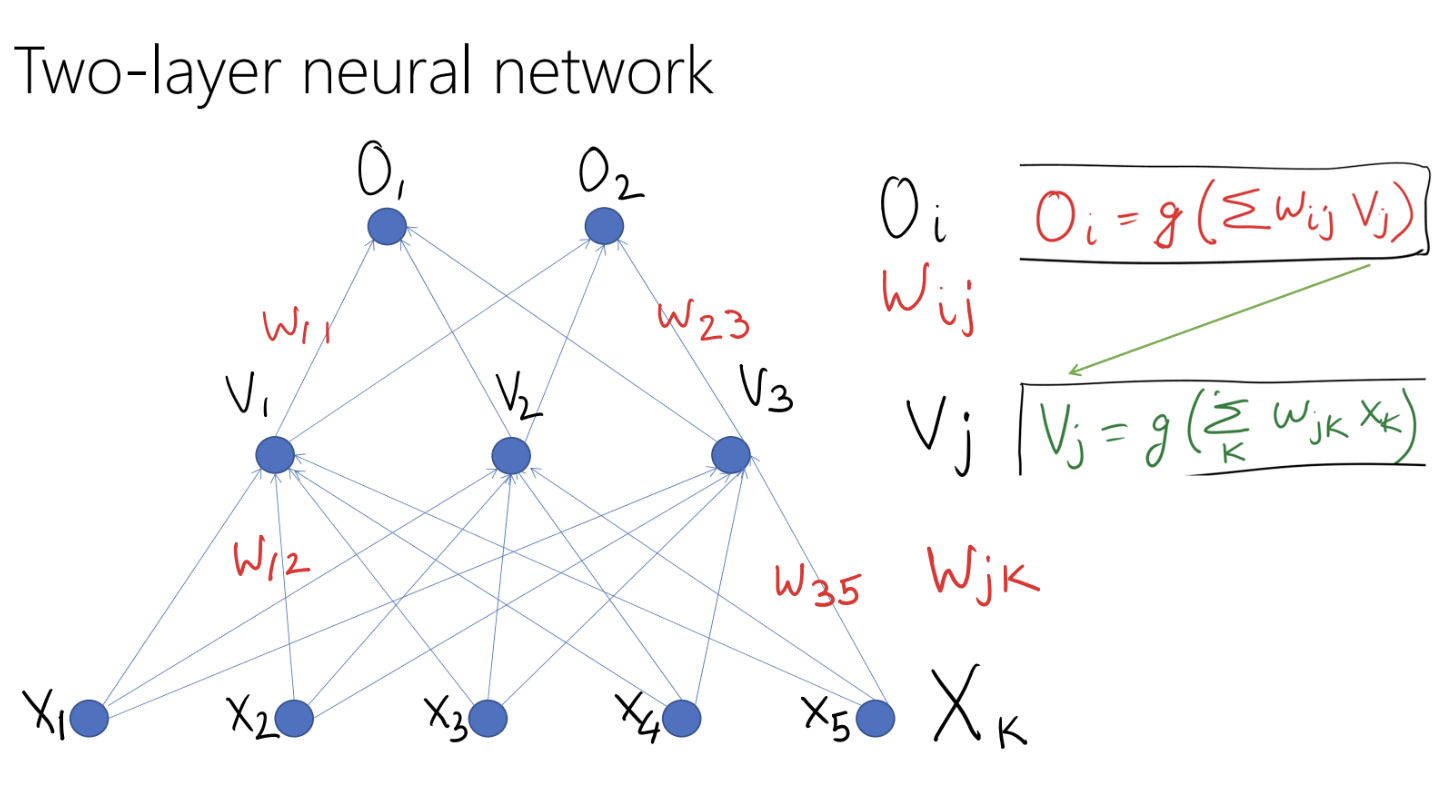
\includegraphics[scale=0.4]{lec-1b.png}
		\end{center}
		Notice how the \( v_i \) gets pushed through our activation function, and so
		does our \( o_i \). Because of the way information is passed from layer to
		layer, this is sometimes called a \textit{feed-forward} neural network.
		If we put it all together, we get:
		\[
			o_i = g\left( \sum_j w_{ij} g\left( \sum_k w_{jk} x_k \right) \right)
		\]
\end{itemize}
\subsection{Training a Neural Network}
\begin{itemize}
	\item At the end of the day, the goal is to find a \( w \), such that \( o_i \)
		is as close as possible to the true label (or true output). If this
		probability is low, then we have a bad setting of the parameters.  
	\item To do this, we can define a loss function \( \mathcal{L}(w) \), and compute
		\( \nabla_w \mathcal{L} \). Then, we update \( w \) by:
		\[
			w_{\text{new}} = w_\text{old} - \eta \nabla_w\mathcal{L}
		\]
		The value of \( \eta \) is called a \textbf{hyperparameter} which we set prior
		to running the training procedure. This process is known as 
		\textbf{gradient descent}. More complicated
		optimization procedures do exist, but they're basically never used in
		practical machine learning.  
	\item Now, the question is, what kind of loss function \( \mathcal{L} \) should
		we use? 
	\item A good choice for a loss function is the likelihood (also known as
		cross-entropy):
		\[
			\mathcal{L} = -\sum_\text{input data}(y_i \ln o_i + (1 - y_i) \ln( 1 -
			o_i) 
		\]
		It turns out, using this as our loss function actually reduces the problem
		directly to logistic regression!  
\end{itemize}

	\section{Maximum Likelihood Estimation}
\begin{itemize}
	\item Recap of last time: we train a neural network by defining a loss function
		\( \mathcal{ L}(w) \), and continuously update our value of \( w \) via
		gradient descent.  
	\item In the equation for \( \mathcal{L} \) that we gave, \( y_i \) represents
		the true label of the data point, and \( o_i \) represents the output of our
		model. 

		If \( o_i \) matches exactly the desired output \( y_i \), then the loss
		function \( \mathcal{L} = 0 \). We only get a positive \( \mathcal{L} \) if
		there is a mismatch between \( y_i \) and \( o_i \).  
	\item For a multi-layer neural network, the same thing applies. We compute the
		gradient with respect too all weights across \textit{all} layers. The
		difference between multi-layer NNs and single layered ones is that the loss
		function \( \mathcal{ L} \) is no longer convex, so you might end up at a
		global optimum instead of a local optimum. 
	\item Generally, computing this gradient is quadratic in the size of \( w \), but
		the back propagation algorithm (a DP-based alg) that allows us to do this in
		linear time instead. This algorithm works for any number of layers.  
\end{itemize}

\subsection{Optimal Classifier}
\begin{itemize}
	\item What is considered the "best" classifier? Theoretically, what is the "best"
		classifier that could be achieved? 

		Here, it's the classifier that minimizes the probability of
		misclassification, or in other words it maximizes the probability that you
		classify correctly. This is called the \textit{Bayes Classifier}. This
		classifier may not have zero training error. 

		However, this is not practical in practice, since we need to know the
		probability distribution of the dataset. It's a circular issue almost, since
		what we want to do anyways is to discover this distribution by looking at our
		data. 
\end{itemize}

\subsection{Error, Validation and Cross-Validation}
\begin{itemize}
	\item There are two main kinds of error that we really care about:

		\textbf{Training Error:} we train a classifier to minimize the training set
		error. We want to minimize the probability of success on this dataset. 
		
		\question{shouldn't we want to \textit{maximize} the probability of success?} 

		\textbf{Test set error:} This is the error from your classifier on a dataset
		that you didn't use to train the model, but a dataset in which you do know
		the true answers for. Part of the game in machine learning is figuring out
		whether you're fooling yourself by making your model seem better than it
		actually is. This test set is also called the validation set. 
	\item So given a dataset, how do we partition the data in such a way that we
		don't run into these issues? One way to do so is through \( k \)-fold cross
		validation. The way it works is we split our dataset up into \( k \) equal
		chunks, and use \( k-1 \) of these to train the model, while the last chunk
		we use to test/validate the model. 
\end{itemize}

\subsection{Maximum Likelihood Estimation (MLE)}
\begin{itemize}
	\item Remember that we want to maximize the likelihood that our model classifies
		things properly, so evidently, MLE is useful here. In terms of our loss, we
		would like to minimize the loss function. 
	\item In supervised learning, we're going to work with a 
		training dataset \( D = \{(x_i, y_i)\}_{i
		= 1}^{N} \). \( x_i \) is a \( d \)-dimensional vector (in the case of our
		images, it would be a \( 28 \times 1 \) vector, and \( y_i \) is some value
		dependent on the problem. If we have a classification, then usually \( y_i \)
		is constrained to two values, \( -1 \) and \( 1 \), but in regression then \(
		y_i\) can be any number, so \( y_i \in \R \) in that case.  

		The only difference between classification and regression is the kind of
		output that we want, whether \( y_i \) is a discrete or continuous variable. 
	\item In unsupervised learning, we lose the notion of \( y_i  \) and instead 
		work only with a dataset \( D = \{x_i\}_{i = 1}^{N} \). In essence, we no
		longer know the right answer, but we do have a bunch of data. In some sense
		it almost feels like a prediction problem, but the model is basically trained
		to learn what actually comes next. This is what Chat-GPT does. 
	\item We also have a \textit{Model class}, written as:
		\[
			f(x \mid w, b) = w^{\top} x + b
		\]
		the model class basically defines the kind of function you are looking for.
		This is also something that we (the creator) have to define for the model. 
		For now, we can think of ML as picking out the best possible model function
		out of this family -- so picking out an optimal \( (w, b) \) in our case --
		but eventually we'll also get into the notion of picking
		a \textit{distribution} of models instead. 

	\item Our learning objective is now to compute:
		\[
			\argmin_{w, b} \sum_{i = 1}^{N}L\left(y_i, f(x_i \mid w, b)\right)
		\]
	\item This only allows us to study statistical models. It means that we treat the
		thing we are trying to estimate as a RV, and we want to know the probability
		distribution of that RV. This phrasing allows us to cast many problems as
		statistical models, which is what makes ML so powerful.   
\end{itemize}

\subsubsection{Quick aside on RVs}
\begin{itemize}
	\item A random variable (RV) is a function \( x \to \R \). Discrete RVs have a
		probability mass function (PMF), and continuous RVs have a probability
		density function (PDF) instead. In terms of normalization, the sum of all
		probabilities in the PMF is 1, and the analogous constraint for PDFs is that
		the integral over the domain is 1. 
	\item Just some RVs as examples: 
		\begin{itemize}
			\item Bernoulli RV: \( P(\text{heads}) = p \), \( P(\text{tails}) = 1 - p
				\). 
			\item Binomial RV: We model \( n \) coin tosses, and count the number of
				heads \( k \):
				\[
					P(x = k) = {n \choose k} p^{k} (1 - p)^{n - k}
				\]
			\item Poisson RV: model the number of mutations \( k \), given that it
				has a mean mutation rate \( \lambda \) over a fixed time interval:
				\[
					P(x = k) = \frac{e^{-\lambda \lambda^{k}}}{k!}
				\]
			\item Gaussian: a continuous RV:
				\[
					p(x) = \frac{1}{\sqrt{2\pi\sigma^2}} \exp\left(
					-\frac{1}{2}\frac{(x - \mu)^2}{\sigma^2} \right)
				\]
		\end{itemize}
	\item So far, we've only looked at univariate distributions. With multivariate
		distributions, the space of outcomes is a vector instead of a scalar. The
		mean becomes a vector also, and the variance now becomes a matrix of
		covariances. We will learn more about this next lecture. 
\end{itemize}

\subsection{MLE Setup}
\begin{itemize}
	\item Given a dataset \( D = \{x_i\}_{i = 1}^{N} \), where each \( x_i \in \R^{d}
		\), and assume a set of distributions on \( \R^{d} \) parametrized by \(
		\theta \), denoted as \( p_{\theta}(x) \). In the case of a Gaussian, then \(
		\theta\) could be the mean and the variance. 
	\item The key assumption we will make is that \( D \) contains sample that
		belongs to one of these distributions in our family: 
		\[
			x_i \sim p_{\hat{\theta}}(x)
		\]
		This assumption also requires that each \( x_i \) is distributed i.i.d. from
		each other. 

		Out goal is to "learn" or estimate the value of \( \theta \) which "pins
		down" the distribution from which the data came. We will define this optimal
		\( \theta \) to be \( \theta_\text{MLE} \). That is, \( \theta_\text{MLE} =
		\argmax_{\theta \in \Theta}p(D \mid \theta) \).   
	\item Note that we have \( p(D \mid \theta) \) instead of the other way around.
		Then because \( D \) is i.i.d, then we have the nice simplification 
		that \( p(\{x_i\}_{i = 1}^{N} \mid \theta) = \prod_{i = 1}^{n} p(x_i \mid
		\theta) \). This lets us break down \( x_i \) away from a summation into a
		product. 
	\item Is there a unique value of \( \theta \) that satisfies MLE? This is not
		always guaranteed! There may be infinitely many solutions that give you the
		maximum likelihood, but there are techniques that allow us to deal with this. 
\end{itemize}
\subsection{MLE Properteis}
\begin{itemize}
	\item \textit{Consistency}: if the data were truly generated by our hypothesis
		family, then as we get more data we're guaranteed that maximizing the
		likelihood is equivalent to finding the true parameters. 
	\item \textit{Statistically efficient}: Given some fixed amount of data, MLE is
		efficient in getting the information it needs out of it.  
	\item The value of \( p(D \mid \theta_{\text{MLE}} \) is invariant to
		reparametrization. Basically, this means that the value of \( p \) doesn't
		depend on the way we look at the problem (or how we parametrized it). Even
		though the returned parameters may change in value, the likelihood does not. 

		Suppose you have a dataset generated from \( N(\mu, \sigma) \), then 
		if you were to draw from \( N(2 + \mu, \sigma) \) instead, then the model
		would find optimality at \( \mu' = \mu - 2 \), but the likelihood doesn't
		change.   
	\item MLE can still yield a parameter estimate even when the data were not
		generated from that family. Usually it's a Gaussian, but we don't know that
		for sure obviously. It doesn't matter how bad your hypothesis class is, it
		will return you a value.  
\end{itemize}
\subsection{Univariate Gaussian Example}
\begin{itemize}
	\item Assume the data is generated from \( X \sim N(x \mid \mu, \sigma^2) \). 
		Now, our goal is to find \( \argmax_{\theta \in \Theta}p(D \mid \mu,
		\sigma^2) \). 
	\item The first step is always to write down the likelihood function:
		\[
			p(D \mid \theta) = p(x_1, \dots, x_N \mid \mu, \sigma^2) = \prod_{i =
			1}^{N}p(x_i \mid \mu, \sigma^2)
		\]
		the product is usually hard to work with, so we'll work with the log
		likelihood instead: 
		\[
			\log p(D \mid \theta) = \sum_{i = 1}^{N}\log p(x_i \mid \mu, \sigma^2) 
		\]
		and because the log function is monotonic, then the value of \(
		\theta_\text{MLE} \) doesn't change when we make this change to the log
		likelihood. 
	\item To solve this maximization problem, we look for stationary points in the
		likelihood, so points where the derivative with respect to \( \mu \) and \(
		\sigma \) are zero. We then also need to confirm that we have a maximum
		point, which we can do by computing the Hessian. In the Gaussian case, the
		Hessian is diagonal, so we can just look at the parameters separately. For
		the mean:
		\begin{align*}
			\pdv{\mu} \sum_{i = 1}^{N}\log p(x_i \mid \mu, \sigma^2) &= \sum_{i}
			\pdv{\mu} \log \left[ \frac{1}{\sqrt{2\pi \sigma^2}}\exp\left(
			-\frac{1}{2\sigma^2}(x_i - \mu)^2 \right) \right] \\
			&= \sum_i \pdv{\mu} \left[-\log(\sqrt{2 \pi\sigma^2}) -
			\frac{1}{2\sigma^2}(x_i- \mu)^2\right] \\ 
			&= \sum_i \left[ 0 + \frac{1}{\sigma^2}(x_i - \mu) \right] 
		\end{align*}
		We now set this to zero, which gives us \( \sum_i x_i = \sum_i \mu \). So
		this tells us that \( \sum_i x_i = N \mu \), or rather \( \mu = \frac{\sum_i
		x_i}{N} \), as expected.
	\item You can do the same thing with the variance, the math is a little more
		complicated but \( \sigma^2 \) does work out. Just take the derivative with
		respect to \( \sigma \), set it to zero, and you will find:
		\[
			\sigma_\text{MLE}^2 = \frac{1}{N}\sum_{i = 1}^{N} (x_i - \mu)^2 = \sigma
		\]
		This is a biased estimate, since the MLE parameter \( \sigma_\text{MLE} \) we
		estimated depends on \( \mu \), which is something we already estimated. As a
		result, we need to change the denominator from a \( \frac{1}{N} \) to 
		a \( \frac{1}{N - 1} \) to account for this loss of a degree of freedom. 

		\question{Truthfully, I don't really understand why changing \( N \) to \( N
		- 1\) corrects for this.}
	\item One drawback of MLE is that it only yields a point estimate of our
		parameter and nothing else. The value of \( \theta \) that maximizes our
		likelihood may be a very sharp spike, which is generally unwanted since it
		means that the model is \textit{very} sensitive to changes in the data. In
		that same vein, a peak which is shorter but doesn't vary as much over a wide
		range of \( \sigma \) may be a better choice. The former case is much more
		likely during overfitting, or basically when you try to fit a 50th order
		polynomial to a function that is represented more by a 4th order.    
\end{itemize}

	\section{Multivariate Gaussians}
\subsection{MLE for Multinomial Distribution}
\begin{itemize}
	\item Now suppose we want to do this for the multinomial distribution. Consider
		flipping a six-sided die, and we want to know the probability of each result.
		That is, \( \theta \) is now a 6-dimensional vector where \( \theta_i \) is
		the probability that the value \( i \) is rolled. 
	\item Given this, we can write \( P(X = k \mid \theta) = \theta_k \). 
	\item Now, since one side is always face up, then we know that \( \sum_k \theta_k
		= 1\), by law of total probability.  
	\item Now, we can write the likelihood:
		\[
			P(D \mid \theta) = P(x_1, \dots, x_N \mid \theta) = \prod_{i = 1}^{N}
			P(x_i \mid \theta) = \prod_{i = 1}^{N}\prod_{k = 1}^{6} \theta_k^{I[x_i =
			k]}
		\]
		the exponent is an indicator variable that tracks whether roll \( i \) is
		equal to \( k \). Otherwise, the exponent evaluates to \( \theta_k^{0} = 1
		\). This is just a weird notational thing that will be helpful later. We can
		then simplify this one more time:
		\[
			P(D \mid \theta) = \prod_{k = 1}^{N}\theta_k^{\sum_{i}^{N} I[x_i = k]} =
			\prod_{k = 1}^{6}\theta_k^{n_k}
		\]
		this last step works because exponents add when we multiply them. Now, we
		take the derivative of this with respect to \( \theta_k \). Now, our MLE
		becomes:
		\[
			\theta_\text{MLE} = \argmax_{\theta \in \Theta} \log p(D \mid \theta) =
			\argmax_{\theta \in \{\Theta \mid 1 = \sum_k \theta_k\}}\sum_{k =
			1}^{6}\log \theta_k^{n_k}
		\]
	\item Now to go ahead and calculate this optimum point, we will use the method of
		lagrange multipliers, because we have a constraint in the problem. 
		We look for \( J(\theta, \lambda) = \log p(D \mid
		\theta) + \lambda(1 - \sum_k \theta_k) \). 

		The rationale for Lagrange multipliers is to take the function we are trying
		to optimize, and add a \( \lambda \) term to it, thereby making it
		"augmented". We now look for stationary points with respect to \( \theta \)
		and \( \lambda \).  
		It's really just there so that we can make sure that our parameters match the
		constraints. It's a way for us to force \( \sum_k \theta_k = 1 \), since
		otherwise \( J(\theta, \lambda) \) will increase in value. The expression for
		\( J \) is:
		\[
			J(\theta, \lambda) = \log p(D \mid \theta) + \lambda \left( 1 - \sum_k
			\theta_k \right) = \sum_{k = 1}^{6}\log \theta_k^{n_k} + \lambda \left( 1
			- \sum_k \theta_k \right)
		\]

	\item Now we take derivatives with respect to \( \lambda \) and \( \theta \).
		Taking this with respect to \( \lambda \):
		\[
			\pdv{J}{\lambda} = 0 \implies 1 = \sum_k \theta_k
		\]
		so we just get our constraint back, not very surprising. 
	\item Now taking the derivative with respect to \( \theta_k \):
		\[
			\pdv{J}{\theta_k} = \pdv{\theta_k} \sum_{k = 1}^{6}\log \theta_k^{n_k} -
			\pdv{\theta_k} \lambda \theta_k = \frac{n_k}{\theta_k} - \lambda = 0
			\implies \theta_k = \frac{n_k}{\lambda}
		\]
		Plugging this into the first equation, we get:
		\[
			1 = \sum_k \theta_k = \sum_k \frac{n_k}{\lambda} \implies \lambda =
			\sum_k n_k = N
		\]
		All together, we have \( \theta_k = \frac{n_k}{N} \). It is also nice (and
		important) to check that \( \theta_k \) is valid, since it ranges between 0
		and 1.  

		\question{Review Lagrange multipliers}
	\item So far, we've been able to use pen and paper to determine what the optimal
		parameters are. This is not the case in general, as many times we will have
		optimization problems that have no closed form solution. To solve this, we
		need something called \textit{iterative optimization}.  
\end{itemize}
\subsection{Multivariate Gaussians}
\begin{itemize}
	\item Recall the univariate Gaussian:
		\[
			p(x; \mu, \sigma^2) = \frac{1}{\sqrt{2\pi \sigma^2}}\exp\left(
			-\frac{1}{2\sigma^2}(x - \mu)^2 \right)
		\]
		The Multivariate Gaussian is just an extension of this, where \( x \in \R^{d}
		\), \( \mu \in \R^{d} \), and \( \Sigma \in \R^{d \times d} \):
		\[
			p(x; \mu, \Sigma) = \frac{1}{(2\pi)^{n / 2} |\Sigma|^{1 / 2}}\exp\left(
			-\frac{1}{2}(x - \mu)^{\top} \Sigma ^{-1} (x - \mu) \right)
		\]
		Despite it looking more complicated, a lot of the things we do with the
		univariate Gaussian work the same in the multivariate case. \( \mu \) used 
		to be a scalar, but now it's a \( 1 \times d \) vector, and the variance \(
		\sigma \) is now this large covariance matrix \( \Sigma \). \( \Sigma \) is a
		PSD (positive semidefinite) matrix, and its inverse is sometimes called the
		precision matrix. 
	\item Why a lecture on MVGs? They are extremely central to modern day ML!
		For instance:
		\begin{itemize}
			\item Classification problems: generative vs. discriminative (we will
				see this in a later lecture)
			\item Unsupervised models: Principal Components Analysis \& autoencoders
				(in a later lecture) 
			\item Advanced Topics: Gaussian Process Regression (beyond the scope of
				this class)
		\end{itemize}
		Even in the case where they aren't useful, because of the central limit
		theorem many datasets we deal with will naturally be normal, and therefore we
		will need to learn how to deal with MVGs. They're also really nice to work
		with (analytically tractable). 
	\item As a teaser, MVGs allow us to reduce dimensions, and it's used to derive the
		steps for Principal Component Analysis (PCA)
\end{itemize}
\subsection{Univariate Gaussians}
\begin{itemize}
	\item To start, let's analyze the case where we have two normal distributions,
		say, the height and weight of humans. By CLT with genetics, we can argue that
		this should be distributed normally, so we have:
		\[
			\text{height} = X_h \sim N(\mu_h, \sigma_h^2) \quad \text{weight} = X_w
			\sim N(\mu_w, \sigma_w^2)
		\]
	\item Now, suppose we want to write the \textit{joint distribution}, how would we
		write this down? One way we can do this is to plot the distribution, and ask
		questions about it. 
		\begin{itemize}
			\item If we computed the mean of the distribution, what would that look
				like? Well, since the height and weight are different parameters, we
				may write it as a vector \( u = [\mu_h, \mu_w] \), for the different
				means. 
			\item How would we describe the spread of the distribution? The
				covariance matrix \( \Sigma \) gives us a way to talk about the
				spread of the distribution when plotted.   
		\end{itemize}
		Ideally, we'd want to use something of the form:
		\[
			p([x_h, x_w]) = N(x_h; \mu_h, \sigma_h^2) N(x_w; \mu_w, \sigma_w^2)
		\]
		\question{At what point have we established that it should even be a product
		of two Gaussians?} 

		But because height and weight are not immediately independent, we cannot
		write it in this form. But, in essence we would like to find a way to
		transform the plot so that we \textit{can} write it in this way.
	\item The trick is so "rotate" the distribution so that the correlation between
		the the two parameters is zero, then we can write it as a product. To compute
		this rotation, we want to multiply by some orthonormal matrix \( Q \) such
		that:
		\[
			\begin{bmatrix} x_1 \\ x_2 \end{bmatrix} = Q \begin{bmatrix} x_h \\ x_w \end{bmatrix}
		\]
		keep this in mind; we will return to this later. 
\end{itemize}

\subsection{Understanding the Covariance Matrix}


\begin{itemize}
	\item Suppose we have two independent Gaussian RVs that are 1D, so we have \( X
		\sim p(x) = N(\mu_1, \sigma_1^2)  \) and \( Y \sim p(y) = N(\mu_2,
		\sigma_2^2) \). Then, we can write the joint distribution:
		\[
			p([x, y]) = \frac{1}{\sqrt{2\pi \sigma_1^2}}\exp\left[
			-\frac{1}{2\sigma_1^2}(x - \mu_1)^2 \right]
			\frac{1}{\sqrt{2\pi \sigma_2^2}}
			\exp\left[ -\frac{1}{2\sigma_2^2}(y - \mu_2)^2 \right]
		\]
	\item We can then write this in matrix form:
		\[
			P(x, y) = \frac{1}{2\pi \sqrt{\sigma_1^2 \sigma_2^2}} 
			\exp\left[-\frac{1}{2} 
				\begin{bmatrix} 
					x - \mu_1 & y - \mu_2
				\end{bmatrix} 
				\begin{bmatrix} 
					\sigma_1^2 & 0 \\ 0 & \sigma_2^2 
				\end{bmatrix}^{-1} 
				\begin{bmatrix} 
					x - \mu_1 \\ y - \mu_2 
			\end{bmatrix} \right]
		\] 
		The intuition for having the \textit{inverse} covariance matrix in the
		exponent is that in a univariate Gaussian, the exponent has a 
		\( \frac{1}{\sigma^2} \) term, so to generalize that we have a 
		\( \frac{1}{\sigma_i^2} \) term, which is achieved using the 
		inverse covariance matrix. 

		\question{Why does this also work for non-diagonal matrices?}  
\end{itemize}

\subsection{Review of Expectations, Variance, Covariance}
\begin{itemize}
	\item Recall that an expectation \( E(X) \) of a random variable \( X \) is
		defined as \( \sum x P(x) \) for discrete and \( \int x P(x) dx \) for
		continuous random variables.  

		There's also the principle of linearity: 
		\[
			E\left(\sum_i \alpha_i x_i\right) = \sum_i \alpha_i E(x_i)
		\]
		this is a guaranteed properly regardless of whether \( x_i \) are
		independent. For products, if \( x_i \) are independent, then we have:
		\[
			E \left( \prod_{i = 1}^{n}x_i \right) = \prod_{i = 1}^{n}E(x_i)
		\]
	\item The Variance of a \( RV \) with mean \( \mu = E(X) \), then the variance is
		defined as \( \Var(X) = E[(X - \mu)^2] \). Expanding htis we get the
		following properties:
		\begin{itemize}
			\item \( \Var(x) = E(X^2) - \mu^2 \)
			\item \( \Var(aX + b) = a^2 \Var(X) \)
			\item If \( x_1, \dots, x_n \) are independent and \( \alpha_1, \dots,
				\alpha_n \) are constants:
				\[
					\Var\left( \sum_i \alpha_i x_i \right) = \sum \alpha_i^2
					\Var(x_i)
				\]
		\end{itemize}
	\item The covariance of two random variables is defined as:
		\[
			\Cov(X, Y) = E\left( (X - E(X)) (Y - E(Y)) \right) = 
			E\left((x - \mu_x)(Y - \mu_y)\right) = E(XY) - E(X)E(Y)
		\]
		We also have \( \Cov(X, X) = \Var(X) \), and if two RVs are independent, then
		\( \Cov(X, Y) = 0 \). 
	\item The correlation is a related parameter, defined as:
		\[
			\Corr(X, Y) = \frac{\Cov(X, Y)}{\sqrt{\Var(X) \Var(Y)}}
		\]
		It's useful to think of it as a "normalized covariance", since the
		correlation is restricted over the domain \( [-1, 1] \). -1 is considered the
		minimum correlation, and 1 is the max correlation, and 0 is no correlation. 
\end{itemize}
\subsection{Return to MVG}
\begin{itemize}
	\item So now we can go back to the covariance matrix, which is a big matrix whose
		\( (i, j) \)-th entry is defined as:
		\[
			\Sigma_{ij} = \Cov(X_i, X_j)
		\]
		From this definition, it's clear that the covariance matrix is always 
		symmetric, since \( \Cov(X, Y) = \Cov(Y, X) \). For Gaussian RVs, it's true
		that if \( \Cov(X, Y) = 0 \) iff \( X, Y \) are independent. \textbf{This is
		not always true, the general case is an "if" case only!}
	\item Now we return to the MVG that we had earlier. We worked through the "baby"
		case of independent RVs, and move to the general case where the covariance
		matrix is not always diagonal. 

		At some fundamental level, the precision matrix is really a descriptor of
		which way the axes in the scatterplot of the data is pointing, and we will
		see how to quantify this by decomposing \( \Sigma^{-1} \) into rotation
		matrices and such. 
	\item Recall the general form for MVGs:
		\[
			p(x; \mu, \Sigma) = \frac{1}{(2\pi)^{n / 2}|\Sigma|} \exp\left(
			-\frac{1}{2}(x -\mu)^{\top} \Sigma^{-1}(x - \mu) \right)
		\]
		the only term we will concern ourselves right now is the quadratic term in
		the exponent. Intuitively, the quadratic term basically maps out the "level
		sets" of the probability distribution, or effectively which values of \( x \)
		give us \( p(x) \) being constant. This is because the equation \( x^{\top}
		\Sigma^{-1} x = c \) basically defines a \( d \)-dimensional ellipse (the
		case is quite easy to see with two dimensions) , with
		which gives us an "orientation" of the Gaussian.  

		\comment{The key takeaway is that the quadratic term defines level sets on
			the MVG, which are in general ellipses. In particular, this description
		comes from the elements of the covariance matrix.}
	\item As an aside, there is a way to transform a general MVG into one whose
		points lie in a circle -- this process is called "sphering" the MVGs. This
		has applications in PCA, advanced linear regressions, etc. 
\end{itemize} 
\subsection{Diagonalizing a Matrix}
\begin{itemize}
	\item The spectral theorem tells us that if we have a symmetric matrix \( A \),
		then we can write \( A = QDQ^{\top} \), where \( Q \) is orthonormal and \( D
		\) is diagonal matrix with real eigenvalues. 

		Since the covariance matrix is symmetric, we can diagonalize it too!
		Moreover, finding the diagonalization is exactly what we need in order to
		"axis align" the MVG, since a remember that a diagonal covariance matrix
		is equivalent to axis alignment.  
	\item There's also another property of MVGs that is important for diagonalization
		called the \textbf{affine property}, which basically states that if \( X \)
		is a set of independent RVs, then if \( Y = AX + \mu \sim N(\mu, \Sigma)\).
		In particular, the covariance matrix of \( Y \) is given by \( A A^{\top}
		\). 

		We can also go the other way around: if \( Y \sim N(\mu, \Sigma) \), then \(
		\Sigma^{- 1 / 2}(Y - \mu) \sim N(0, I)\). This is analogous to the that you
		can always transform a Gaussian to one with zero mean and unit variance.  
\end{itemize}

	\section{Linear Regression}
\begin{itemize}
	\item Today we will make use of MLE that we've been learning, and also our
		knowledge about Gaussians.
\end{itemize}
\subsection{Regression}
\begin{itemize}
	\item It's a form of supervised learning, where we have data pairs \( D = \{(x_i,
		y_i)\} \) where \( x_i \) may be discrete or continuous. \( x_i \) may also
		be scalar/vector, but \( y_i \) is always a scalar.  
	\item Formally, we want to find \( p(y \mid x) \), or essentially the conditional
		pdf for the data points \( y \) given the values \( x \). 
	\item We usually think about getting a "point" prediction of a model which is
		just given by \( \hat{y} = E_y[p(Y \mid X = x)] \). We will explore this for
		a while, then back out of this and look at the other forms later.
	\item When you usually think about regression you probably think of a regression
		line -- one way to think about the regression line is that it also gives us a
		probability for every given value of \( x \), and the best fit line is the
		one that maximizes this probability.  
	\item What are some strategies we could use to estimate \( p(y \mid x) \)? 
		\begin{enumerate}[label=\arabic*.]
			\item \textbf{Generative:} Estimate \( p(x, y \mid \theta) \), then we can use the fitted
				model to compute \( p(y \mid x, \hat{\theta}) \). 

				Basically, we can use what we built earlier with MLEs to calculate \(
				p(x, y \mid \theta)\), then we can use that to compute \( p(y \mid x)
				\). 


				In particular, we can compute:
				\[
					p(y \mid x, \theta) = \frac{p(y, x \mid \hat{\theta})}{p(x,
					\hat{\theta})} = \frac{p(y, x \mid \hat{\theta})}{\int_y (y,
				x \mid \hat{\theta}) \diff y}
				\]

				\question{For MLEs, don't we have \( p(y, x \mid \theta) \) (or
					rather, we find the \( \theta \) that optimizes the data given the
					parameter, which is not what we're doing here when we write \( p(x, y
					\mid \theta) \)?}
			\item \textbf{Discriminative:} We can assume the inputs to be fixed, and only the output is a
				random variable. That is, we try to directly model \( p(y \mid x,
				\hat{\theta}) \). 

				The advantage of this approach versus the previous one is that we
				don't treat \( x \) as an RV. In some cases, if we
				\textit{absolutely} don't understand the distribution of \( x \), it
				may be a bad idea make assumptions about it (e.g. treat it as a
				Gaussian RV). This is a deep question and we won't go into this
				further.   
		\end{enumerate}
\end{itemize}
\subsection{Linear Regression}
\begin{itemize}
	\item This takes the discriminative approach to generate the prediction. IN
		particular, the predictions will be a linear function of the parameters --
		this is what the "linear" in linear regression refers to. For instance:
		\[
			\hat{y} = E_y[p(y \mid x)] = w^{\top} x + w_0
		\]
		\( w \) is the parameters, \( x \) is the input features, and \( w_0 \) is
		the "bias". This is considered linear, since \( y \) is linear in terms 
		of \( x \). 
	\item One thing we will do is that instead of a bias, we will make an extra
		features that always equals 1, and instead use \( x' = [x, 1] \). This allows
		us to basically keep track of the bias without having to write it out
		explicitly -- we can also write \( \hat{y} = w^{\top} x' \) instead.  
	\item Linear models are also very useful! Instead of just computing \( \hat{y} =
		w^{\top} x\), we can also \textit{augment} our feature space, and also track,
		say, a quadratic term. So, we can also have \( \hat{y} = w^{\top}[x, x^2] \)
		for instance, and in fact we can augment by any polynomial. This allows our
		linear regression to "fit" to any polynomial. 

		This process of taking the original input space and "expanding" this out in
		terms of predetermined functions is called a \textit{basis expansion}.
		Suppose you had \( x \in \R^{2} = [x_1, x_2] \), then we can basis expand
		quadratically:
		\[
			[1, x_1, x_2, x_1x_2, x_1^2, x_2^2] \in \R^{6}
		\]
		this can all come from \( x \)! For \( d = 1 \), then the polynomial
		expansions is the set \( [1, x, x^2, \dots, x^{n}] \).  
	\item These are predetermined functions that we always know ahead of time and
		plug \( x \) into, so this gives us a lot of freedom in what we want to fit
		to. As a notational thing, we will write \( \hat{y} = w^{\top} \Phi(x) \)
		instead, where \( \Phi(x) \) is the basis expansion.    

		Note that \( \Phi(x) \) can be \textit{literally anything}! We can pick
		anything from just the standard polynomial basis to even the Fourier basis
		for our regression. It's all up to us. 
	\item As a sneak peek, we can actually \textit{learn} the basis functions, but we
		won't go into this today. 
	\item For the rest of this lecture, we will just assume \( \hat{y} =
		w^{\top} x \) for now. 
\end{itemize}
\subsection{Specific Linear Regression}
\begin{itemize}
	\item So far, we know that \( \hat{y} = w^{\top} x \). What should we use for \(
		p(y \mid x)\)? 
	\item For linear regression, the assumption we will use is that for each \( x \),
		there is a Gaussian distribution for \( y \), that shares the same variance.
		So, \( p(y \mid x) = N(y \mid w^{\top} x, \sigma^2) \). This is equivalent to
		writing \( Y = w^{\top} x + \epsilon \), where \( \epsilon \sim N(0,
		\sigma^2)\) is a Gaussian. 

		\comment{I don't like the notation here, instead I think it may be better to
			write \( p(y \mid x) = N(w^{\top} x, \sigma^2) \), the given symbol makes
		no sense in a distribution definition.} 
	\item We can then rearrange this to \( Y - w^{\top} x = \epsilon \sim N(0,
		\sigma^2) \). \( \epsilon \) is also sometimes called the \textit{residuals},
		which we assume to be normally distributed with equal variance. 

		\comment{As an aside, there are other distributions called heavy-tail
			distributions, which favor values along the tails much more than the
			Gaussian. This is just to show that the residuals can realistically be
		any distribution, we will stick to Gaussians in this lecture.}  
	\item Now we fit the parameters \( w \). We will use MLE. Here, \(
		\theta_\text{MLE} = (w_\text{MLE}, \sigma^2_\text{MLE})\). This is very
		similar to what we did two weeks ago. We will take the log-likelihood, so
		this is equal to:
		\[
			\theta_\text{MLE} = \argmax_{w, \sigma^2} \sum_{i = 1}^{n} \log p(y_i
			\mid x_i, \theta) = \argmax_{w, \sigma^2} \sum_{i = 1}^{n} \log\left(
			\frac{1}{\sqrt{2\pi\sigma^2}} \right) - \frac{1}{2\sigma^2} \sum_{i =
		1}^{n}(y_i - w^{\top} x_i)^2
		\]
		This last line comes from the assumption that each \( y_i \) can be modeled
		by a normal distribution with mean \( w^{\top} x_i \) and variance \(
		\sigma^2 \).  
	\item Note that here the estimation of \( w \) doesn't depend on \( \sigma \), so
		maximizing \( w \) is the same as finding:
		\[
			\argmin_w \sum_{i = 1}^{n}(y_i - w^{\top} x_i)^2 = \argmin_w \sum_{i =
			1}^{n}(y_i - \hat{y}_i)^2
		\]
		this is the same least-squares function that you've been taught in previous
		classes.  
	\item Now to actually find \( w \). If we vectorize this equation, we can write
		this as \( y - Aw \), where \( A \) is called the "design matrix" and
		represents the vector of inputs \( x \). With this in mind, we can then
		rewrite the loss as \( \argmin_w \|y - Aw\|_2^2 \). 

		The loss can then be written as:
		\[
			\mathcal{L} = \|y - Aw\|_2^2 = y^{\top} y - 2w^{\top} A^{\top} y +
			w^{\top} A^{\top} Aw
		\] 
		and we want to set \( \pdv{L}{w} = 0 \). Computing the derivative (using
		vector calculus, \question{review this}), we have:
		\[
			\nabla_w \mathcal{L} = -A^{\top} y + A^{\top} A w \implies w = (A^{\top}
			A)^{-1}A^{\top} y
		\]
		Then, we just need to check that this is a critical point, which we can do by
		looking at the Hessian. The hessian matrix is \( \nabla_w^2 \mathcal{L} =
		2A^{\top} A \), and we require that this is positive definite (PD) in order
		for it to be minimized. This is achieved when \( A \) is full rank.   
	\item The \( \sigma^2_\text{MLE} \) for this is really just the exact same thing,
		and we will end up getting 
		\[
			\sigma^2 = \frac{1}{n}\sum_i(y_i - w^{\top} x)^2
		\]
		exactly as we expect. 
	\item There is also a geometric viewpoint of this, but this is much more rigid,
		and overall seems to be a "weaker" interpretation of least squares than the
		statistical approach. 
\end{itemize}

	\section{Linear Regression II}
\begin{itemize}
	\item Recall from last time we talked about Gaussian Linear Regression, where we
		wanted to estimate \( \hat{y} =- \E_Y[p(y \mid x)] = w^{\top} x \). We
		assumed that the residuals were Gaussian distributed, and from this math we
		were able to recover the standard equations of linear regression. 

		We wrote out \( \mathcal{L}_w = (Y - Aw)^{\top} (y - Aw) \), and then set \(
		\pdv{\mathcal{ L}}{w} = 0\) to solve for \( w^{*} \). From this, we obtained
		\( w_\text{MLE} = (A^{\top} A)^{-1} A^{\top} y \), and \( \sigma_\text{MLE}^2
		= \frac{1}{n}\sum_i (y_i - w^{\top} x)^2\)
	\item However, one major problem in this approach is that \( A^{\top} A \) may
		not be invertible, which is the case when the features are not linearly
		independent. For instance, if you have more features than data points, then
		this will be the case. When it's not invertible, then there are infinitely
		many good equations for \( w_\text{MLE} \), and this is called an
		\textit{underdetermined system}. 
	\item There are two ways for us to fix this: 
		\begin{enumerate}[label=\arabic*.]
			\item Remove features (via some type of heuristic) in the problem 
				until the problem is linearly
				independent. This is called "feature selection". This is an entire
				area of ML that people are actively researching. 
			\item Add constraints to the system to "tighten the system". This is
				called "regularization". In some sense, we add constraints to limit
				the number of degrees of freedom from the system. 

				Here, we keep the same number of parameters, but add constraints on
				the system so that we remove some of the freedom offered by these
				features. 
		\end{enumerate}
\end{itemize}

\subsection{Intuition for infinite solutions}
\begin{itemize}
	\item To illustrate this, suppose you have two features that are linearly
		dependent, so \( \alpha x_1 = x_2 \). 
	\item Suppose now that you found one \( \hat{w} \). Then, for any training data
		point, we have \( \hat{y} = x^{\top} \hat{w} \) to be our point prediction.
		We will now show that there are infinitely many \( \hat{w} \) that give us
		the same prediction. If we expand this out:
		\[
			\hat{y} = \begin{bmatrix} x_1 & x_2  \end{bmatrix} 
			\begin{bmatrix} \hat{w}_1 \\ \hat{w}_2 \end{bmatrix}
			= \hat{w}_1 x_1 + \hat{w}_2 (\alpha x_1) = (\hat{w}_1 + \hat{w}_2 \alpha +
			\beta - \beta)x_1 = (\hat{w}_1 + \beta) x_1 + (\hat{w}_2 \alpha - \beta)
			\frac{x_2}{\alpha} = 
			\begin{bmatrix}  x_1 & x_2 \end{bmatrix}
			\underbrace{\begin{bmatrix} \hat{w}_1 + \beta \\ \frac{\hat{w}_2 \alpha -
			\beta}{\alpha} \end{bmatrix}}_{\hat{w}'}
		\]
		and this gives us a different value of \( \hat{w} = \hat{w}' \) that also gives the same
		prediction \( \hat{y} \). As a result, there are an infinite number of
		"optimal" \( \hat{w} \) that gives the same prediction. 
	\item The one that the Moore-Penrose chooses is the one that has the smallest
		norm. Why might we want to choose this one? 

		The reason we may want to choose this is because usually, solutions with
		small norms affect our model in a more "uniform" way, where it is not greatly
		influenced by small perturbations to our input (imagine adding a little
		amount \( \delta \) to \( x \), and checking how our model reacts to it). 
		Keeping the norm small is one
		way we can ensure that this principle is maintained.  
	\item What about the case where our design matrix is full rank? Is there any
		reason we may want to put a constraint on \( \|w\| \)?   
\end{itemize}
\subsection{L2 Regularized Linear Regression} 
\begin{itemize}
	\item We will learn two systems, today, L2 and L1 regularization. These just
		refer to the different norms that we will use to choose our optimal \(
		\hat{w} \). 
	\item In L2 regression, our loss function is:
		\[
			\mathcal{L} = (y - Aw)^{\top}(y - Aw) + \lambda \|w\|_2^2
		\]
		This is also sometimes called "ridge" regression, they mean the same thing. 
	\item In te Bayesian model approach, what we will do is establish a \textit{prior
		distribution} on the parameters, \( p(\theta)  \). Then, we want to compute
		the posterior distribution, \( p(\theta \mid D) \). 

		The \( p(\theta) \) is something that we can establish ahead of time (without
		looking at the data), and then with this we can calculate \( p(\theta \mid D)
		\). 
	\item Then, the predictive distribution is given by:
		\[
			p(y \mid x) = \int_\theta p(y\mid x, \theta) p(\theta \mid D) \diff \theta
		\]
		This is generally done using Bayes rule:
		\[
			p(\theta \mid D) = \frac{p(D \mid \theta) p(\theta)}{p(D)}
		\]
		This is exceedingly dfficult to do in practice! This is not really something
		that we will touch on further due to its difficulty. 
	\item We will be "lazy", so instead of using normalized Bayesian probability (as
		described here), we will just compute \( \argmax_\theta p(\theta \mid D) \),
		and that will be our optimal \( \theta \). This is called maximum \textit{a
		posteriori} (MAP) estimation.  

		\comment{Conceptually, the way we solve this is the exact same as MLE, except
			we now multiply by a \( p(\theta) \) term. This selects favorably for
			some probability models over others; you can equivalently think of MLE as
			the case where there is no preference for any particular model, since \(
		p(\theta) = 1\).}
\end{itemize}
\subsection{MAP Estimation}
\begin{itemize}
	\item Again, now we are calculating \( \theta_\text{MAP} = \argmax_\theta
		p(\theta \mid D) \). By Bayes' rule, we have:
		\[
			\argmax_\theta \frac{p(D \mid \theta) p(\theta)}{p(D)} = \argmax_\theta
			p(D \mid \theta) p(\theta)
		\]
		recall that \( p(\theta) \) is our "prior" density for \( \theta \), and \(
		p(D \mid \theta) \) is the posterior distribution.
	\item The prior \( p(w) \) that corresponds to L2 regression is \( p(w) = N(w; 0,
		\lambda I)\). So, using this, let's try to find \( w_\text{MAP} \). First, we
		take the logarithm, so we have:
		\begin{align*}
			w_\text{MAP} &= \argmax_w \log p(D \mid w) p(w)\\
						 &= \argmax_w \log p(D \mid
			w) + \log N(w; 0, \lambda I)\\
			&= \argmax_w \sum_{i = 1}^{N} \log N(y_i \mid w^{\top} x_i, \sigma^2) +
			\log N(w \mid 0, \lambda I) \\ 
			&= \argmin_w \frac{1}{2\sigma^2}(y - Aw)^{\top}(y - Aw) - \sum_{i =
			1}^{d}\log\left[\frac{1}{\sqrt{2 \pi \lambda}} \exp \left( -
			\frac{w_i^2}{2 \lambda} \right)\right]
		\end{align*}
		Note that we haven't taken the logarithm of the second expressino yet so
		that's why the signs don't match yet. Then, after more simplification we get:
		\[
			w_\text{MAP} = \argmin_w (y - Aw)^{\top}(y - Aw) + \lambda' \|w\|_2^2
		\]
		for \( \lambda' = \frac{\sigma^2}{\lambda} \). 

	\item You will almost always benefit from doing this as opposed to ordinary
		linear regression -- this approach helps a lot with numerical stability as
		well as guaranteeing uniqueness.    
	\item The MAP solution just involves taking the partial derivative and set it to
		zero, which we've already done on the homework. Here, we have:
		\[
			\nabla_w \mathcal{L}_\text{MAP} = -2A^{\top} y + 2A^{\top} Aw + 2 \lambda
			I w \implies w^{*} = (A^{\top} A + \lambda I)^{-1} A^{\top} y 
		\]
		if \( \lambda > 0 \), then we can always guarantee that the matrix \(
		A^{\top} A + \lambda I \) is invertible.  
	\item The effect of \( \lambda \) is also important here. As you increase \(
		\lambda \), the norm of \( w^{*} \) gets increasingly smaller. Practically,
		how should we set \( \lambda \)? 

		\question{yeah how do you do this? the slides don't really go into detail
		about this.}
\end{itemize}

\subsection{Lasso regression}
\begin{itemize}
	\item This is using the L1 norm, which means that:
		\[
			w_{L_1} = \argmin_w (y - Aw)^{\top} (y - Aw) + \lambda \|w\|_1
		\]
		This penalty tends to choose sparse \( w \) over other ones, because the
		penalty favors points on the axes compared to other points. L1 regression is
		more likely to hit a contour on one of the axes, and thus it has a higher
		chance of setting some parameters to exactly zero. 

		By contrast, the L2 penalty looks like a ball, so there is no such bias. 
	\item There is also a way for us to derive L1 regression, by using a Laplacian
		prior:
		\[
			p(w) = \exp(-\lambda' \|w\|_1)
		\]
	\item There are some advantages to Lasso over ridge. Because of Lasso's tendency
		to sparsity, sometimes it is best to just turn one of the parameters off,
		which is sometimes favorable. On the other hand, when you have two parameters
		that are highly correlated, then Lasso is bad because in choosing an optimum
		it might just turn one completely off. 
	\item People have also combined these two together, into a regression called
		"elastic net regression". This is a middleground between the two regression
		techniques, but we won't go into the details here. 
\end{itemize}

	\section{Classification: Generative and Discriminative}
\begin{itemize}
	\item Classification is a fundamentally different problem than a regression
		problem. IN a regression problem, we usually deal with a dataset \( y_i \in
		\R \), but in regression, the output is not a real number but rather a label:
		\[
			\mathcal{X} \to \mathcal{Y} \in \{0, \dots, K - 1\}
		\]
	\item The labels can be binary, or also perhaps more complicated. The MNIST
		dataset is not binary, since we have images and we want to classify them into
		the digits 0-9, for example. 
	\item In general, the problem is phrased like this: given a dataset \( \{(x_i,
		y_i)\}_{i = 1}^{n} \), we are interested in \textit{learning} the
		classification 
		\[
			f_{\theta}: \mathcal{X} \to \{0, \dots K - 1\}
		\]
\end{itemize}
\subsection{Bayes' Rule}
\begin{itemize}
	\item In the context of classification, it's used to transform class-conditional
		probabilities into posterior probabilities. In particular,
		\begin{align*}
			p(0 \mid x) &= \frac{p(x \mid 0) p(0)}{p(x)}\\
			p(1 \mid x) &=  \frac{p(x \mid 1) p(1)}{p(x)} 
		\end{align*}
		The variables \( p(x \mid 0), p(x \mid 1) \) are called the
		\textit{class-conditional probabitlities}. The value of \( p(x) \) is
		determined using the law of total probability:
		\[
			p(x) = p(x \mid 0) p(0) + p(x \mid 1) p(1)
		\]
	\item The hard part is finding the right class-conditional probability --
		we always have to ask ourselves, what kind of distribution do we expect? The
		answer to this is usually motivated by our prior knowledge about the
		population; maybe half of the population we expect to tend one way, so our
		distribution should reflect that. 
	\item If we map the posterior probabilities, we'll get a graph like this: 

		\begin{center}
			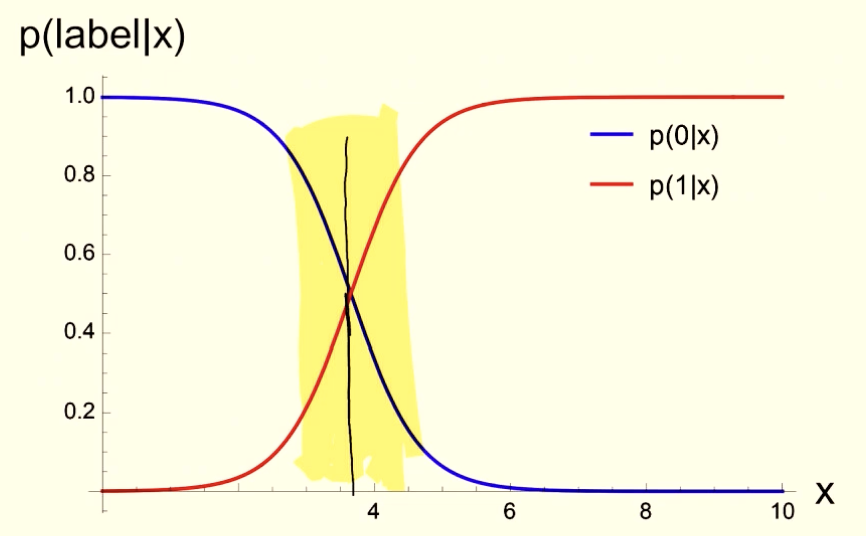
\includegraphics[scale=0.5]{lec-6a.png}
		\end{center}
		But what should we do in the region highlighted in yellow? This is a
		gray-area, where we aren't 100\% certain that we should classify one way or
		the other.     
		\begin{itemize}
			\item One thing we can do here is look at the intersection between these
				two curves, call it \( x^{*} \), and basically classify:
				\[
					f_{\theta}(x) = \begin{cases}
						0 & x < x^{*}\\
						1 & x \geq x^{*}
					\end{cases}
				\]
			\item This is a somewhat reasonable rule to follow, since this allows us
				to potentially reduce the probability of classifying incorrectly at
				least from a probabilistic standpoint.  
		\end{itemize}
	\item In general, we want to pick a value of \( k \) (the classification) 
		such that \( p(k \mid x) \)
		is maximal. Equivalently, this means that we want to reduce the probability
		of error:
		\[
			P(\text{error}) = \int p(\text{error}\mid x) p(x) \diff x 
		\]
		In doing this, you are treating false positives and false negatives with eual
		weight. However, this is not always the case. For instance, if you're in the
		medical field, false negatives can be much more detrimental than false
		positives, often fatal, so in cases like that we should be more careful about
		how we classify things.  

		\question{What if you just classify the error as the probability of
			\textit{misclassificaiton}? It seems that we're phrasing "error" in terms
		of testing positive, which isn't the best method of classification?}

		\comment{It seems like they haven't covered exactly how to quantify error
		just yet.} 
\end{itemize}

\subsection{Ways of Building Classifiers}
\begin{itemize}
	\item There are three main ways we can build classifiers: 
		\begin{enumerate}[label=\arabic*.]
			\item \textbf{Generative:} to model the conditional probabilities \( p(x
				\mid k)\), then use Bayes' rule to get \( p(k \mid x) \). This
				requires you to somehow model the prior \( p(k) \). 
			\item \textbf{Discriminative:} Model \( p(k \mid x) \) directly. 
			\item \textbf{Find Decision Boundaries:} Directly solve for the
				boundaries \( f : \mathcal{X} \to \{0, \dots, K - 1\} \).  

				This approach has the drawback that you lose information about how
				close your data point is to any of the boundaries, which means that
				you lose the ability to quantify your model's uncertainty in the
				system.  
		\end{enumerate}
\end{itemize}
\subsection{Logistic Regression}
\begin{itemize}
	\item Logistic regression is a classification method, where we model the
		posterior probability by a logistic function:
		\[
			p(k = 0 \mid x) = \frac{1}{1 + e^{-(\theta_1 x + \theta_0)}}
		\]
		We can also extend this to \( K \) classes, but for now we will talk about
		two classes 0 and 1.   
	\item If the class-conditional density \( p(x \mid \{0, 1\}) \) is Gaussian, then
		we claim that the posterior probability will be a logistic function 
		in \( z = \theta_1x + \theta_0 \). 

		\question{What is \( \theta_1, \theta_0 \)? Are these fitted parameters, or
		what?} 

		\answer{No, \( \theta_1 \) and \( \theta_0 \) are parameters that you can
			mathematically solve for. You can solve for these variables by literally
			letting \( P(x \mid k) \sim N(\mu_k, \sigma)\) (assume the variances are the
		same), and work out the math via Bayes' rule. }
	\item In our case then, \( z \) is a linear function of \( x \), plus a bias term
		\( \theta_0 \). This is called an "affine" function. 
	\item We can then generalize this to multivariate Gaussians, where we assume:
		\[
			P(X \mid k) \sim N(\mu_k, \Sigma)
		\]
		here \( \Sigma \) is the covariance matrix. 

		\comment{Review the proof in the slides, ask about what's happening.} 
	\item Intuitively, we want a sigmoid (logistic) function to model our
		probabilities because it's very nice -- the probability is always between 0
		and 1, so it's always well-behaved, and it's also smooth so there's nice
		properties there as well. 
\end{itemize}
\subsection{Modeling the Posterior Probability Distribution}
\begin{itemize}
	\item To give a preview, here's what we're going to do:

		We basically set up a label \( Y \in \{0, 1\} \) to be a Bernoulli random
		variable (for simplicity I think), with its probability parameter so we have:
		\[
			P(Y = 1 \mid x) = \frac{1}{1 + \exp(- \theta^{\top} x - \theta_0)} :=
			\mu(x)
		\]
	\item In the binary case, we can take \( y \) to denote the values taken on by
		the random variables, so:
		\[
			p(y \mid x) = \mu(x)^{y} (1 - \mu(x))^{1 - y}
		\]
		(this is just law of total probability applied to Bernoulli RVs). 
	\item In the next lecture, we will learn how to estimate \( \theta_1, \theta_0 \)
		using MLE methods. 
\end{itemize}

	\section{Logistic Regression \& Neural Networks}
\begin{itemize}
	\item Last time, we saw how the logistic equation came out of assuming Gaussian
		class-conditional variables. This lecture, we will continue that exploration,
		and see how we can use MLE to get the logistic function.
	\item In summary, we found that the posterior takes the form:
		\[
			p(k \mid x) = \frac{1}{1 + e^{-z}}
		\]
		where \( z \) is a \textbf{linear} function \( z = \theta^{\top} x + \theta_0
		\). Here, \( \theta \) is a parameter that depends on \( \{\mu_k\}_{k =
		1}^{K} \) and \( \Sigma \).  
		
		This method of determining \( p(k \mid x) \) is called the
		\textbf{generative} approach. Now, we will talk about the discriminative
		approach.  

	\question{My understanding is that there is a generative and discriminative
	approach to classification problems and regression problems, is that true?}      

	\answer{Probably? This approach probably works for anything where you have data
	and you want to find parameters that describe the data well.}  
\end{itemize}

\subsection{Multi-Class Classification}
\begin{itemize}
	\item First, we will start by looking at how our two-class classification can be
		generalized to \( K \) classes. We will start with the generative approach,
		because that's what we did last time.  
	\item We first start by writing out the class-conditional probability. This is
		assumed to be Gaussian (like before), though note that this isn't the only
		function we could pick.
		\[
			p(x \mid k) \sim N(\mu_k, \Sigma)
		\]
		Here, \( \mu_k \in \R^{d} \) and \( \Sigma \in \R^{d \times d} \). To find
		the posterior distribution, we will invoke Bayes' rule:
		\[
			p(k \mid x) = \frac{p(x \mid k) p(x)}{p(k)} = \frac{p(x \mid k)
			p(k)}{\sum_{i = 1}^{k}p(x \mid j) p(j)}
		\]
		Here, we will now rewrite this in a "nicer" way, by letting \( a_k = \log p(x
		\mid k) p(k) \), so we may write:
		\[
			p(k \mid x) = \frac{e^{a_k}}{\sum_{j = 1}^{K}e^{a_j}}
		\]
		More explicitly, we have:
		\[
			a_k = (\Sigma^{-1} \mu_k)^{\top} x - \frac{1}{2}\mu_k^{\top} \Sigma^{-1}
			\mu_k + \log p(k)
		\]
		which you can get just by multiplying it out and collecting the terms
		appropriately. Here, we will denote \( \theta_k = \Sigma^{-1} \mu_k \), and \(
		\theta_{0, k} \) is just the remainder of the expression. This then allows us to
		write \( a_k = \theta_k^{\top} x + \theta_{0, k} \), which is linear as desired. 

		\comment{As an aside, this mapping:
			\[
				(a_1, \dots, a_k) \mapsto \left( \frac{e^{a_1}}{\sum e^{a_j}}, \dots,
				\frac{e^{a_k}}{\sum e^{a_j}}\right)
			\]
			is called the \textit{softmax function}. In particular, if we have \( a_k \gg
			a_j\), then the softmax mapping will basically map this \( n \)-tuple into a
		basis vector.}
\end{itemize}

\subsection{Discriminative Learning}
\begin{itemize}
	\item We're given this hypothesis that \( p_{\theta}(0 \mid x) \) has the functional
		form:
		\[
			p_{\theta}(0 \mid x) = \frac{1}{1 + e^{-(\theta^{\top} x + \theta_0)}}
		\]
		As before, we will use the log-likelihood, and given that we assume i.i.d
		conditions we have a product which turns into a sum in the logarithm.   
	\item Given this form, the likelihood is then given by:
		\[
			\log\left( p_z^{y} (1 - p_z)^{1 - y} \right)
		\]
		\question{work out what \( z \) is in terms of \( \theta, x \) and the other
		stuff to make it match the form above.} 
		Here, \( z \) depends on \( \theta \) and \( p \) only depends on \( z \). In
		order to find the optimal \( \theta \), then this is a quantity we'd like to
		maximize. At the same time, the loss is something we'd like to minimize, so
		we can define the loss to be the negative of this. 
		\[
			\mathcal{L}(\theta) = -y \log p_z - (1 - y)\log(1 - p_z)
		\]
	\item To find the maximum then, we can take \( \nabla_{\theta}\mathcal{L}(\theta)
		\) and we get:
		\begin{equation}
			\label{lec6}
			\nabla_{\theta}\mathcal{L}(\theta) = \left( -y \frac{p_z(1 - p_z)}{p_z} +
			(1 - y) \frac{p_z(1 - p_z)}{1 - p_z}\right)\nabla_{\theta}z = (p_z - y)
			\nabla_{\theta}z
		\end{equation}
		To get this form, we note that since \( p_z \) is a sigmoid, then we have:
		\[
			\partial_z p_z = \frac{e^{-z}}{(1 + e^{-z})^2} = p_z( 1 - p_z)
		\]
		The \( \nabla_{\theta}z \) term is very deep -- in linear this term is just
		equal to \( x \), but in more complex systems (for instance, in deep
		learning), it need not be linear. 
\end{itemize}
\comment{The rest of this lecture was a \textit{very} light intro to neural nets by
	talking about neurons and human cells so I didn't feel like writing that stuff
	down. All you really need to know is that neural networks are just simplified models
of biological neural nets.} 

	\section{Gradient Descent and Backpropagation}
\begin{itemize}
	\item Last lecture, we visited the logistic regression, talked about the softmax
		function, and also looked at the log-likelihood loss for gradient descent.
		We were also able to interpret the gradient \(
		\nabla_{\theta}\mathcal{L}(\theta) \) geometrically in terms of how we update
		parameters. 
	\item The gradient is written as:
		\[
			\nabla_{\theta}\mathcal{L}(\theta) = (p_z - y) \nabla_{\theta}z 
		\]
		we write \( p_z - y \) as the "error" term -- so if we were to make an
		incorrect classification, then we would have a nonzero loss.  
\end{itemize}
\subsection{Single-Layer Neural Networks}
\begin{itemize}
	\item As a single layer, we can represent the neural network as follows:
		\begin{center}
			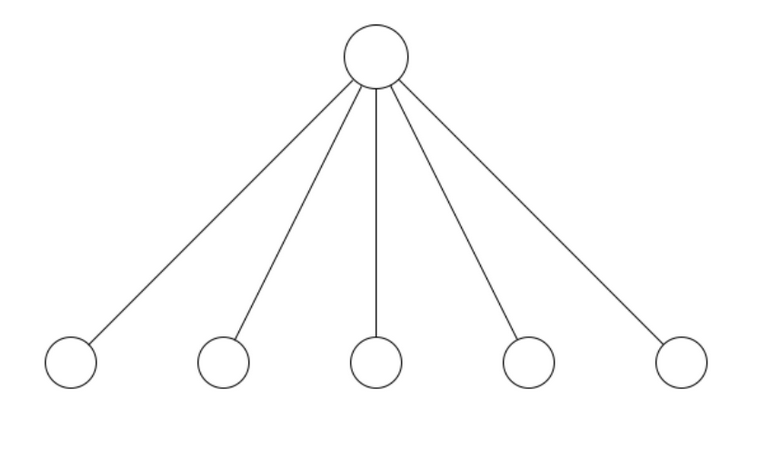
\includegraphics[scale=0.6]{images/one-layer-NN.png}
		\end{center}
		The bottom layer is the input \( x^{(0)} \in \R^{d}\), and the top layer is 
		the output \( x^{(1)} \). Along each "edge" between \( x_i^{(0)} \) and \(
		x^{(1)} \), there are weights \( \theta_{ji} \) which we multiply by their
		respective \( x_i^{(0)} \) to get their contribution in \( x^{(1)} \). 
		So, to calcualte \( x^{(1)} \), we have:
		\[
			x^{(1)} = g\left( \sum_{i} \theta_{ji}^{(1)}x_i^{(0)} \right)
		\]
		\( g(z) \) is called the \textit{activation function}. 
		There are many different values of \( g(z) \) that you can choose: you can
		use a sigmoid, a linear function, or like \( \max(z, 0) \). This last one is
		called ReLU. Another fun one is \( g(z) = \frac{z}{1 + e^{-z}} \), and is
		called SiLU. 
\end{itemize}
\subsection{Two-Layer Neural Networks}
\begin{itemize}
	\item As their name describes, this is the case where you have two layers:
		\begin{center}
			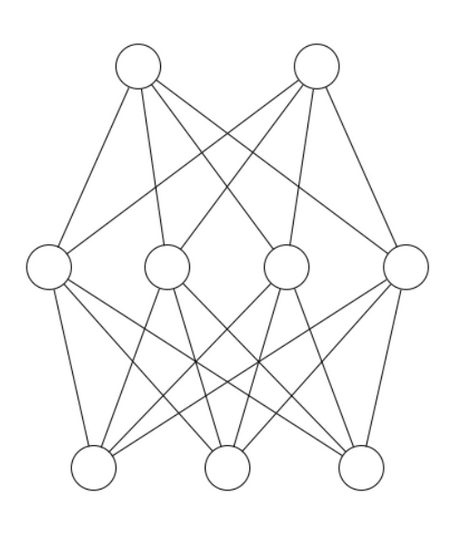
\includegraphics[scale=0.6]{images/two-layer-NN.png}
		\end{center}
		with the following functions:
		\begin{align*}
			x_k^{(2)} = g\left( \sum_j \theta_{kj}^{(2)} x_{j}^{(1)} \right)\\
			x_{j}^{(1)} = g\left( \sum \theta_{ji}^{(0)} x_i^{(0)} \right)
		\end{align*}
		basically, we dot each \( x_j^{(m)} \) with \( \theta_{kj} \) to get \(
		x_k^{(m + 1)} \), then apply the activation function to get the result of the
		next layer. 
	\item In general, each layer has an arbitrary number of layers, so the first
		layer has dimension \( d_0 \) and the second layer \( d_1 \), etc.. You also
		can change \( g \) at every layer, but because this is usually hard to track
		people just stick to a single value of \( g \). 
	\item We also add a unit node that is set to 1 on each layer, which is connected
		to every node in the next layer. This is called the \textit{bias}. 

		\question{why do we introduce the bias?} 

		\answer{We introduce the bias for the same reason we do it in linear
			regression -- we don't want to necessarily restrict the neural network at
			each layer to \textit{have to} pass through \( (0, 0) \), so the bias
		corrects for that.}
	\item We can then generalize this and make our neural net as complicated as we
		want, with the only restriction being that we don't allow any loops. 
	\item As an aside, if you have a function \( f: \R^{d_1} \to \R^{d_2} \), this
		architecture that we've built is actually enough to approximate \( f \) to
		arbitrary accuracy. 
	\item The last layer is also something that is given to us by the problem. If
		we're doing regression which is given by a real value, then the last layer is
		a single node. If we're doing \( K \) classification, then the last layer
		will have dimension \( K \). 
\end{itemize}
\subsection{Gradient Descent}
\begin{itemize}
	\item Before we go any further, we will prove a theorem first:

		\begin{theorem}
			The gradient \( \nabla f(\theta) \) of a function 
			\( f : \Theta \to \R \) at any point \( \theta \) is perpendicular to the
			level set of \( f \) at that point. 
		\end{theorem}

		\begin{proof}
			We define a path \( t \) on the level set in question. Because
			it is a level set, then we know that the level set has the property that
			\( f \) is constant over that set. Thus, for any path \(
			\theta(t) \) we define over the level set, we will have \( \partial_t
			f(\theta(t)) = 0 \). Expanding this:
			\[
				0 = \partial_t f(\theta(t)) 
				= \pdv{f}{\theta_1} \pdv{\theta_1}{t} + \dots
				\pdv{f}{\theta_m} \pdv{\theta_m}{t} = (\nabla f)\cdot \vec v 
			\]
			so, we can only have that \( \vec v \) (or the tangent to the path over
			the level set) is perpendicular to \( \nabla f \), as desired.   
		\end{proof}
	\item Now, consider \( f(\theta) = \frac{\theta^2}{2\alpha} \). This is a
		parabola, where \( \alpha \) controls the "flatness" of the parabola:
		\begin{center}
			\begin{tikzpicture}[domain=-2:2, samples=100]
				\draw[color=blue] plot (\x, {(\x)^2/2}) node[above right]
					{\( \alpha = 1\)} ;
				\draw[color=black] plot (\x, {(\x)^2/8});
				\draw[color=black] plot (\x, {(\x)^2});
				\draw (-5, 0) -- (5, 0);
				\draw (0, -1) -- (0, 5);
			\end{tikzpicture}
		\end{center}
		We ask the question, what does gradient descent look like here?\footnote{As a
		reminder, gradient descent is just a way to "walk along the curve".} Based on
		the rule of gradient descent, we have:
		\[
			\theta_{t + 1} = \theta_t - \epsilon \nabla f(\theta) = \theta_t -
			\epsilon \frac{\theta_t}{\alpha} = \left( 1 - \frac{\epsilon}{\alpha}
			\right) \theta_t
		\]
		Now, suppose you started with some \( \theta_1 \), and we ran this \( t \)
		times. The closed form of \( \theta_t \) is:
		\[
			\theta_t = \left( 1 - \frac{\epsilon}{\alpha} \right)^{t} \theta_1
		\]
		If \( \epsilon < \alpha \), then \( \theta_t \) decreases and approaches zero. 
		If \( \epsilon > \alpha \), then \( \theta_t \) increases, and eventually
		diverges. If \( \epsilon = \alpha \), then after a single step, 
		we've already reached the minimum value so \( \theta_2 = \theta_{min} \). 
	\item So, hopefully this analysis gives some intuition on how the size of 
		\( \epsilon \) that we choose is dependent on \( \alpha \). If \( \alpha \)
		is small, then we likewise need to choose a small \( \epsilon \) in order to
		prevent our function from diverging. 

		Now imagine this in higher dimensions, where the curvature of your level set
		varies depending on where you are on the level set. Then, the \( \epsilon \)
		you choose is constrained by the smallest value of \( \alpha \) that exists
		in the shape.  
\end{itemize}
\subsection{Stochastic Gradient Descent}
\begin{itemize}
	\item Now we will talk about stochastic gradient descent. Here, we will consider
		a loss function, which is expressed as the sum of individual losses:
		\[
			\mathcal{L}(\theta) = \sum_{i = 1}^{n} \mathcal{L}_i(\theta)
		\]
		where \( \mathcal{L}_i(\theta) \) is the loss for any particular data point:
		\[
			\mathcal{L}_i(\theta) = \mathcal{L}(x_i, y_i, \theta)
		\]
		The reason it takes this form is because of the i.i.d. assumption, so that
		when we compute the loss it just ends up being a sum over the loss of an
		individual point. Then, it follows that:
		\[
			L_{i}(\theta) = - \log p_{\theta}(x_i, y_i)
		\]
	\item So far, we've seen two methods to solve this:
		\begin{itemize}
			\item Linear regression:
				\[
					-\log p_{\theta}(x_i, y_i) = \frac{1}{2 \sigma^2} (y_i -
					\theta^{\top} x_i^{(0)} + \text{const.}
				\]
				\question{why do you have a \( \frac{1}{2\sigma^2} \) term here?}

				\answer{The exponent in the Gaussian has a \( \frac{1}{2\sigma^2} \)
				term.} 
			\item Logistic Regression:
				\[
					-\log p_{\theta}(x_i, y_i) = -y_i \log g(\theta^{\top} x_i^{(0)})
					- (1 - y_i) \log(1 - g(\theta^{\top} x_i^{(0)})) + \text{const.}
				\]
		\end{itemize}
	\item Stochastic gradient descent is a process in which you use one of these
		regression losses, and perform the following update scheme:
		\[
			\theta_{t + 1} = \theta_t - \epsilon_t \nabla_{\theta}\mathcal{L}(x_i,
			y_i, \theta)
		\]
		Here, \( \epsilon_t \) is chosen at random, typically without replacement.
		In essence, we are picking at random how large our \( \epsilon \) is.  
	\item This approach has worked in practice -- we usually see that in high
		dimensions the loss is "dominated" by saddle points (so false minima), and
		the variance introduced by SGD seems to avoid these points. 

		That said, it has also been shown that the noise hurts us when we get close
		to the optimal point, slowing the algorithm down. There is a compromise that
		you can make, which is to divide the dataset into \( b \) batches of size \(
		n / b\), where for each batch you compute the loss and perform the
		corresponding update.  
\end{itemize}

	\section{Backpropagation and Gradient Descent II}
\subsection{Summary of Previous Lecture}
\begin{itemize}
	\item Neural Networks. In particular, we said that
		an \( L \)-layer (feed forward) neural network is described as:
		\begin{align*}
			a_j^{(\ell)} &= \sum_{i \in [d_{l - 1}]} \theta_{ji}^{(\ell)} x_i^{(\ell -
				1)}\\ 
					x_{j}^{\ell} &= g_\ell(a_j^{(\ell)})\\
			g_\ell &: \R \to \R
		\end{align*}
		\( a \) is usually called the "preactivation". \( g \) is a function that we
		have a lot of freedom over (linear, nonlinear, etc.). By convention however,
		we say that \( g_L(z) = z \) is a linear function, and \( g_{\ell} = g \) is
		typically held fixed. 
	\item The loss \( \mathcal{L}(\theta) \) is a function which we typically will
		formulate as the negative log likelihood. 
		\[
			\mathcal{L} = -\log p_\theta
		\]
		Keep in mind that the loss doesn't have to be defined in terms of the
		log-likelihood, but we will stick to doing this for now.  
	\item Gradient-based optimization: we minimize the loss \( \mathcal{L}(\theta) \)
		using gradient descent:
		\[
			\theta_{t + 1} = \theta_t - \epsilon_t \nabla_{\theta_t}
			\mathcal{L}(\theta_t)
		\]
		For neural networks, what is this loss? For 1-layer neural networks, this has 
		the form:
		\[
			\partial_{\theta_{ki}^{(1)}}\mathcal{L} = \partial_{a_k^{(L)}}\mathcal{L}
			\partial_{\theta_{ki}^{(L)}}a_k^{(L)}
		\]
		\question{When you talk about loss in this context, are you talking about the
		loss at a particular layer, or the loss of the network as a whole?}  

		\answer{The loss of the network as a whole is not well-defined, so this is
		probably the loss at layer.} 
\end{itemize}
\subsection{Loss for \( K \)-classification}
\begin{itemize}
	\item If we have more than two classes, how do we compute the loss? We will show
		that
		\[
			\mathcal{L} = -\sum_{k \in [K]} y_k \log \frac{\exp(a_k^{(L)})}{Z}
		\]
		where \( Z \) is defined as the normalization:
		\[
		Z = \sum_{k \in [K]} \exp(a_k^{(L)})
		\]
		This loss \( \mathcal{L} \) should be read as log over the product of \( p_k
		\), and we "normalize" \( p_k \) using the softmax function. So in its
		unsimplified form, the following is what we're dealing with: 
		\[
			\mathcal{L } = -\log \prod_{k = 1}^{K} p_k^{y_k}
		\]
	\item Combining this with what we have for linear regression, you can actually
		derive the answer. In the linear case, we have:
		\[
			\partial a_{1}^{(L)} \mathcal{L} = a_1^{(L)} - y
		\]
		so for \( k \) output neurons, we can just generalize this to \( k \):
		\[
			\partial_{a_k^{(L)}} \mathcal{L} = p_k - y_k
		\]
		\question{He keeps mentioning one-hot encoding, what does this mean again?}
	\item To convince ourselves further let's actually work through the math for this
		problem. We are interested in \( \Delta_k = \pdv{L}{a_k^{(L)}} \). We will
		just write \( a_k^{(L)} \) as \( a_k \) just for ease of notation. Writing
		out the partial derivative, we hvae:
		\[
			\Delta_k = \pdv{\mathcal{L}}{a_k} = -\pdv{a_k} \left( \sum_j y_j \log
			\frac{e^{a_j}}{Z} \right)
		\]
		\( Z \) is the normalization. For the denominator, because it's a sum over
		all \( e^{a_j} \), then only the \( e^{a_k} \) term survives when we take \(
		\pdv{Z}{a_k}\). Now, let \( p_j = \frac{e^{a_j}}{Z} \). Then:
		\[
			\pdv{p_j}{a_k} = \begin{cases}
				\frac{e^{a_j}}{Z} - \frac{e^{a_j}e^{a_j}}{Z^2} & j = k\\
				-\frac{e^{a_j}e^{a_k}}{Z^2} & j \neq k
			\end{cases}
		\]
		we can write this out in a more simplified form:
		\[
			\pdv{p_j}{a_k} = p_j(\delta_{jk} p_k)
		\]
		where \( \delta_{jk} \) is the kronecker delta. Thus, we have:
		\begin{align*}
			\Delta_k &= - \sum_{j} \frac{y_j}{p_j} \pdv{p_j}{a_k}\\
			&= -\sum_j y_j \frac{1}{p_j}p_j(\delta_{jk} - p_k) \\ 
			&= -y_k + \left( \sum_j y_j \right) p_k\\
			&= p_k - y_k
		\end{align*}
		The last step we use the fact that \( \sum_j y_j = 1\), which is the case
		because it's zero for every class except the one we know it belongs to. 
\end{itemize}
\subsection{Generalized Loss}
\begin{itemize}
	\item We previously defined the error with respect to the last layer, but now
		let's try to generalize this to all layers. That is, we want to derive:
		\[
			\partial_{\theta_{ji}^{(l)}}\mathcal{L}
		\]
		for all the weights \( \theta \).  
	\item There is an algorithm called \textit{backpropagation} that gives us a way
		to compute the loss at the top layer \( \ell = L \) and propagate it all the
		way down to \( \ell = 1 \). This algorithm is \( O(m) \), which is better
		than the naive approach of computing the Taylor expansion which runs in \(
		O(m^2) \). 
\end{itemize}
\subsection{Backpropagation}
\begin{itemize}
	\item So our objective is to compute the loss with respect to an arbitrary
		parameter, or \( \pdv{\mathcal{L}}{\theta_{ji}} \) from a neuron in layer \(
		\ell \) to \( \ell - 1 \). 
	\item Recall that the preactivation and the post-activation is written as:
		\[
			a_{j}^{(\ell)} = \sum_i \theta_{ji}^{(\ell)} x_i^{(\ell - 1)} \quad 
			 x_i^{(\ell - 1)} = g(a_i^{(\ell - 1)}) 
		\]
		and the loss (depending on the type of model we use) is defined as:
		\[
			\mathcal{L} = \begin{cases}
				\frac{1}{2}( y - a^{(L)})^2 & \text{Gaussian}\\
				- y \log \sigma(a^{(L)}) - (1 - y) \log(1 - a^{(L)}) &\text{logistic}\\ 
				-\sum_k y_k \log \frac{a_k^{(L)}}{Z} & \text{multiclass}
			\end{cases}
		\]
		And we also have the general formula from earlier:
		\[
			\pdv{\mathcal{L}}{\theta_{ji}^{(\ell)}} = \pdv{\mathcal{L}}{a_j^{(\ell)}}
			\pdv{a_j^{(\ell)}}{\theta_{ji}^{(\ell)}}
		\]
		The second term is very simple because \( a_j^{(\ell)} \) is linear in terms
		of \( \theta_{ji}^{(\ell)} \), so the partial derivative just gives us \(
		x_i^{(\ell - 1)} \). For the first term, we can use our single-layer neural
		network to motivate the form. We know that the last layer is expressed in
		terms of the layers below, so to generalize this notion we introduce a chain
		rule because we have an activation function \( g \): 
		\[
			\Delta_j^{(\ell)} := \pdv{\mathcal{L}}{a_j^{(\ell)}} = \sum_k
			\underbrace{\pdv{\mathcal{L}}{a_k^{(\ell + 1)}}}_{\Delta_k^{(\ell + 1)}}
			\pdv{a_k^{(\ell + 1)}}{a_j^{(\ell)}}
		\]
		well we've just abstracted this out to the next layer up since the
		
		first term in the sum is just the loss in the previous layer. For the second
		term in the chain rule, we know that
		\[
			a_{k}^{(\ell + 1)} = \sum_i \theta_{ik}^{(\ell+1)} g(a_j^{(\ell)})
		\]
		so the derivative is:
		\[
			\pdv{a_k^{(\ell + 1)}}{a_j^{(\ell)}} = \theta_{kj}^{(\ell + 1)}
				g'(a_j^{(\ell)})
		\]
		\question{He mentioned something about a kronecker delta, where does it
		appear?} 

		\answer{We are taking the derivative with respect to a particular \(
			a_j^{(\ell)} \), so only one of these terms survive. This is why you
		have a kronecker delta and only one term in the result.} 

		So finally, we can write:
		\[
			\Delta_j^{(\ell)} = \left(\sum_{k \in [d_{l + 1}]} \Delta_k^{(\ell +
			1)}\theta_{kj}^{(\ell + 1)}\right)g'(a_j^{(\ell)})
		\]
	\item To interpret this, the error at any particular layer is determined by the
		accumulation of the errors at the layer above -- this is why we call this
		"propagating" the errors back through the network. This is a recursive
		formula, which takes \( O(m) \) time for \( m \) layers.
	\item In general, if you follow the structure of layer-by-layer computation, then
		this takes linear time, but if you have skip connections (connections between
		layer \( \ell \) and \( \ell - 2 \), for example), then this algorithm would
		take longer. 
\end{itemize}

	\section{CNNs, ResNets, Batch Normalization}
\subsection{Summary of Last Lecture}
\begin{itemize}
	\item The structure of a neural network: we described the mathematical structure
		of a neural network and how each neuron behaves at every step:
		\begin{align*}
			a_j^{(\ell)} &= \sum_{i \in [d_{\ell - 1}]} \theta_{ji}^{(\ell)}x_i^{(\ell
			- 1)}\\
			x_j^{(\ell)} &= g_\ell(a_j^{(\ell)}) 
		\end{align*}
	\item For maximum likelihood learning, we denote the total loss as the sum of the
		individual losses: 
		\[
			\mathcal{L}(\theta) = \sum_i \mathcal{L}_i(\theta) = \sum_i
			\mathcal{L}(f_{\theta}(x_i), y_i)
		\]
	\item Stochastic Gradient Descent (SGD): in its purest form, defined by the
		updates
		\[
			\theta_{t + 1} = \theta_t - \epsilon_t
			\nabla_{\theta_t}\mathcal{L}(\theta_t)
		\]
		where we select an \( \epsilon_t \) at random at each iteration \( t \). 
	\item Backpropagation: we learned of an \( O(m) \) algorithm to calculate the
		gradient of the loss throughout the neural net:
		\[
			\Delta_j^{(\ell)} = \left( \sum_{k \in [d_{\ell + 1}]} \Delta_k^{(\ell +
			1)} \theta_{kj}^{(\ell + 1)} \right)g'(a_j^{(\ell)})
		\]
\end{itemize}
\subsection{Convolutional Neural Networks (CNN)}
\begin{itemize}
	\item Firstly, fully connected neural networks are parameter hungry. Usually,
		too many parameters leads to overfitting of the data, which we know to be
		suboptimal.
	\item The motivation for CNNs comes from our desire to incorporate our "inductive
		bias" into the neural net. Inductive bias is our desire to force the neural
		network to learn certain aspects about the data. 

		In our naive approach, if we wanted to forcefully change some parameters \(
		\theta \), then the network would respond in an unpredictable way because of
		its complexity. So, in order to control the neural networks in a way, we turn
		to convolutional neural networks.  
\end{itemize}

\subsubsection{Invariance and Equivariance}
\begin{itemize}
	\item They are both defined with respect to a particular transformation.
	\item As an example, consider a translation \( T \):
		\[
			\begin{tikzcd}[sep = 30]
				x \arrow[r] \arrow[d, "f_\theta"] & T(x) \arrow[d, "f_\theta"] \\
				f_{\theta}(x)  &  f_\theta(T(x))	
			\end{tikzcd}
		\]
		the idea is that with our classification, we would like to have \(
		f_\theta(x) = f_\theta(T(x)) \). In this case, we call this
		\textbf{invariance.}
	\item On the other hand, if we have \( f_{\theta}(T(x)) = T(f_{\theta}(x)) \),
		then this operation is called \textbf{equivariance}. 

		In general, because the spaces (dimensions) in which \( x \) and \( T(x) \)
		live in may be different, what we really want in general is:
		\[
			f_{\theta}(T_x(x)) = T_y(f_{\theta}(x))
		\]
		In the case where \( T_x = T_y \) we have the earlier form. 
\end{itemize}
\subsubsection{Structure of a CNN}
\begin{itemize}
	\item In a CNN, the operation from each layer to the next is a convolution, and
		no longer a dot product between the vector \( \theta \) at layer \( \ell \)
		and your weights. That is, 
		\[
			a^{(1)}(i_1, i_2) = \sum_{j_1 \in [F]} \sum_{j_2 \in [F]} x^{(0)}(i_1 +
			j_1, i_2 + j_2) \theta(j_1, j_2)
		\]
		so now, \( \theta \) is a 2-dimensional kernel we use to compute the
		convolution. This also means that each neuron is only connected to the
		neurons in the previous layer by the size of the convolution only.    

		\question{what does the bias actually mean in this case then? Is it some
		constant matrix \( \theta_0 \)?}

		\answer{No, you do the convolution as normal, then add a bias \( b \) at the
		very end.}
	\item Note that the filter at each layer doesn't have to be the same. If you were
		processing an image, one filter could be a horizontal gradient, and the other
		could be a vertical gradient. This is allowed.  
	\item In the case of image processing, you may also need to take your
		convolutions channel-wise because your input is RGB.  
	\item In general, visualizing the first layer of your network is relatively easy,
		because it's just a collection of the images you've learned.

		\question{Is the first layer the output layer or the first layer through your
		convolution?}
	\item Some technical terms related to neural nets: 
	\begin{itemize}
		\item \textbf{Padding:} When you do convolution on the edges, you may need to pad
			the edges with zeros (or some other value) so that the kernel completely
			overlaps with your matrix. In general, convolving a \( (W \times W) \) matrix
			with an \( (F \times F) \) filter, then you get a \( (W - F + 1)
			\)-dimensional matrix. 
		\item \textbf{Pooling:} You take the elements in a certain window of the matrix
			(say, the top left), and take the value according to some defined function.
			In the case of max-pooling, you take the max value, for example. 
	\end{itemize}
	\item When we finish training our model using SGD (or other methods), we can then
		look at the learned model by computing \( \nabla_x a_i^{(\ell)}(x;
		\hat{\theta}) \). Basically, we are looking for the behavior of the neural
		net to small changes in the data. 
	\item One thing we find when training neural networks is that the depth of the
		neural net doesn't always lead to a better result, and is a result of the
		vanishing gradient. 

		\question{What is this vanishing gradient really mean here?} 

		\answer{Consider logistic regression, where your activation function is the
			sigmoid. You want to maximize the probability, which forces you to be in
		a regime where there are very small gradients. So, you hit a wall.}


		\comment{Aside on vanishing gradients:
			Consider a function:
			\[
				f(x) = \left( \prod_{i = 1}^{n}w_i \right)x
			\]
			and you have individual gradients:
			\[
				\pdv{\mathcal{L}}{w^{(2)}} 
				= \pdv{\mathcal{L}}{x^{(3)}}
				\pdv{x^{(3)}}{w^{(2)}}
		\]
	The reason vanishing gradients happen is because you multiply many of these terms
together -- and as a result, you're getting a \textit{really} small term, and this
leads to vanishing gradients.}
\end{itemize}

\subsection{ResNets}
\begin{itemize}
	\item One way to deal with the limitations of neural networks is to use "skip
		connections", or basically connect the previous layer directly to the next
		layer. That is, we have:
		\[
			x^{(\ell + 1)} = \mathcal{F}_{\ell + 1}(x^{(\ell)}) + x^{(\ell)}
		\]
		compared to what we had before (only the \( \mathcal{F}_{\ell +
		1}(x^{(\ell)}) \) the residual \( x^{(\ell)} \) term (not sure)

		\question{so what does the residual term do that allows you to bypass the
		learning barrier?} 

		\answer{It solves the issue of vanishing gradients, because the gradient of
		the last step directly influences the first step.} 
	\item As a result, deeper ResNets actually do perform progressively better.    
\end{itemize}

\subsection{Batch Normalization}
\begin{itemize}
	\item When you want to train a neural net, and you don't want inputs from
		different layers of the network to be in different ranges. Because of the way
		backpropagation works (each next layer is dependent on the previous one),
		then you'd like all the gradients and networks to live in similar ranges so
		that you don't get random spikes for no reason.
	\item To accomplish this, you normalize each hidden layer in the same way you
		normalize the input data! That is, in each batch, we can compute the
		statistics of the batch:
		\[
			\mu_B = \frac{1}{n}\sum_{i \in [b]} x_i, \quad \sigma_B = \frac{1}{n}
			\sum_{i \in [b]}(x_i - \mu)^2
		\]
		then normalize each layer based on the statistics of the batch. That is, for
		each node in the neural network, we then have:
		\[
			x^{(\ell)} \leftarrow \frac{x^{(\ell)} - \mu_B}{\sigma_B + \epsilon}
		\]
		this normalizes each \( x^{(\ell)} \) in each batch so make sure that the
		ranges are consistent across each layer. \question{Remember: this is done at
			\textit{every layer}, so you compute \( \mu_B \) and \( \sigma_B \) for
		each layer, and normalize it.} 
	\item You also want to augment \( x^{(\ell)} \) by learned \( \gamma, \beta \):
		\[
			x^{(\ell)} \leftarrow \gamma x^{(\ell)}+ \beta
		\]
		\question{and why do you do this?}

		\answer{Don't worry about it, it's not important.}
\end{itemize}

	\section{Recurrent NNs, Attention \& Transformers}
\subsection{Sequence-to-Sequence Models}
\begin{itemize}
	\item To motivate the later topics in this lecture, one question we should answer
		is how we deal with variable length inputs. In the case of protein folding,
		you have different length sequences for different proteins, so how do you get
		your neural net to predict parameters like the stability, or structure of the
		protein?

		In the most interesting case, your output is contingent on the length of your
		input. This is the case in language translation. 
	\item In general, you need a way to handle variable length inputs, and models
		that do this are called \textbf{sequence-to-sequence models}.
	\item Let's first consider only variable length inputs, so we have something
		like:
		\begin{align*}
			x_1 &= (x_{1, 1}, x_{1, 2}, x_{1, 3}, x_{1, 4})\\
			x_2 &= (x_{2, 1}, x_{2, 2}, x_{2, 3}) \\ 
			x_3 &= (x_{3, 1}, x_{3, 2}, x_{3, 3}, x_{3, 4}, x_{3, 5}) 
		\end{align*}
		because you want to have variable length inputs, you can't just feed the
		neural network the entire \( x_1 \) because then you lose the ability to have
		variable length. 
	\item One possible way you could do this is to feed each dimension of the input
		vector sequentially. That is, for \( x_1 \), we first feed it in \( x_{1, 1}
		\), then \( x_{1, 2} \), then \( x_{1, 3} \), etc. As a diagram:
		\begin{center}
			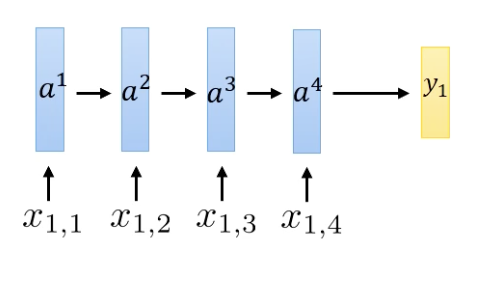
\includegraphics[scale=0.7]{images/lec11-1.png}
		\end{center}
		so, the output \( a^{3} \) hinges on the output \( a^2 \), and so on.
		For inputs with shorter length, we can just prepend a bunch of zeros, which
		does nothing to the data.
	\item In principle, this would work, but the major problem with this direct
		approach is that the number of layers in your network is equal to the length
		of the largest input. If you have very few long inputs, then the model won't
		be very good at predicting the long inputs because there isn't enough data
		out there. 

		To fix this, we tie the layer parameters together, which is called a
		recurrent neural network. It's called recurrent because each \( a^{\ell} \)
		depends recursively on \( a^{\ell - 1} \). 
	\item Something else you could do is to have an output for each input, and
		"decode" the output from that specific layer. The computation is the same,
		the only thing we've changed is that we're decoding the information at every
		step. 
	\item You could also use what's called an \textbf{autoregressive model}, which
		uses the output of the previous iteration to generate the next output. This
		is what ChatGPT does. 

		\question{How is this model different than the first one?} 

		\answer{You are getting the output at every step here, in the first type
			you're not. In other words, you're getting the output of each next word,
		which is generated based on the prevoius word.} 
	\item From this process, hopefully it's clear that there's this general setup
		going on: you have an encoder that "encodes" the input data, and a decoder
		that you run through your neural network to decode the output. That is, the
		general structure could look something like this:
		\begin{center}
			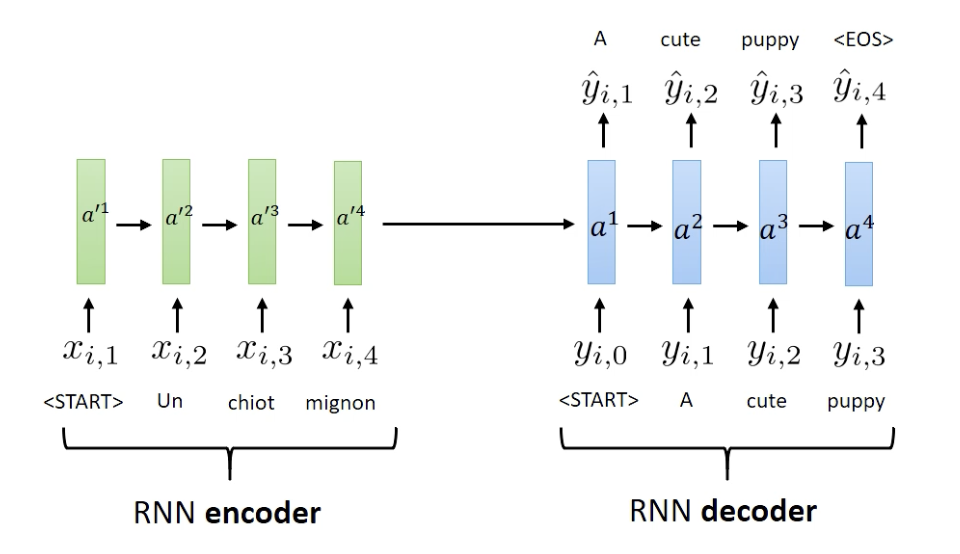
\includegraphics[scale=0.6]{images/lec11-2.png}
		\end{center}
		Note that the RNN encoder could be replaced by a CNN encoder if we were
		dealing with images. Point is, you have a neural network that
		\textit{encodes} the input data, and a decoder that \textit{decodes} the
		data. 

		The encoder translates the input into a "content vector" that describes the
		content, then the RNN decoder does the actual translation.    
\end{itemize}
\subsection{RNN Bottleneck, Attention}
\begin{itemize}
	\item One major problem with this encoder-decoder structure is the transition
		between the encoder and the decoder, called the bottleneck. In essence, if
		you have very long recurrences, then the earlier features that are passed in
		tend to get washed out the longer your recurrence goes. 

		This is the motivation for solutions that involve attention and transformers.
	\item Suppose you don't want all the information to be bottlenecked by the last
		output of the encoder, is there a way we can just translate intermediate
		outputs? The answer is yes, via attention. 
	\item Imagine the standard recurrent neural network (image below), and 
		you're trying to decode \( s_2 \). 
		\begin{center}
			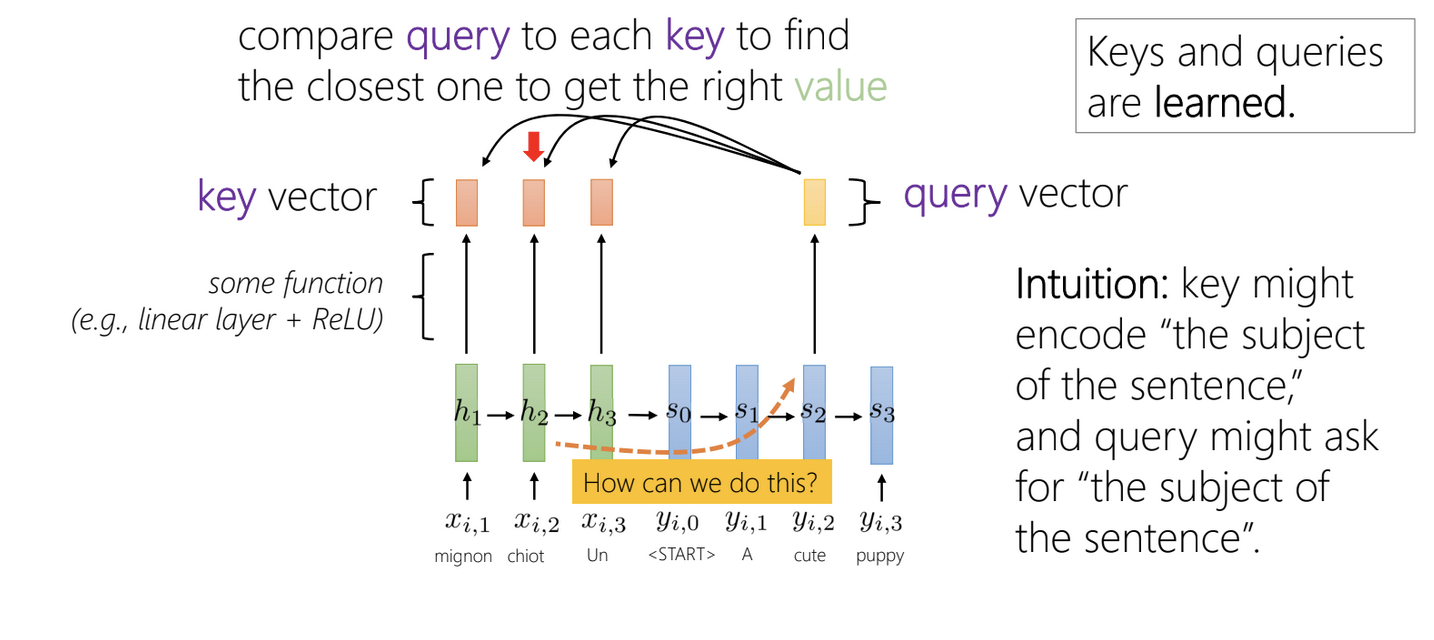
\includegraphics[scale=0.5]{images/lec11-3.png}
		\end{center}
		we can generate a query vector based on the hidden state at \( s_2 \), that
		allows us to query back in time and look for matches. This is a probabilistic
		lookup, so it picks the one that has the highest similarity, based on some
		heuristic (maybe a dot product or something).     

		\comment{The intuition to have is that if you're trying to decode the subject
			of the sentence, the query vector goes back in time and looks for the
		subject of the sentence from the encoder.}
	\item Refer to the diagram below:
		\begin{center}
			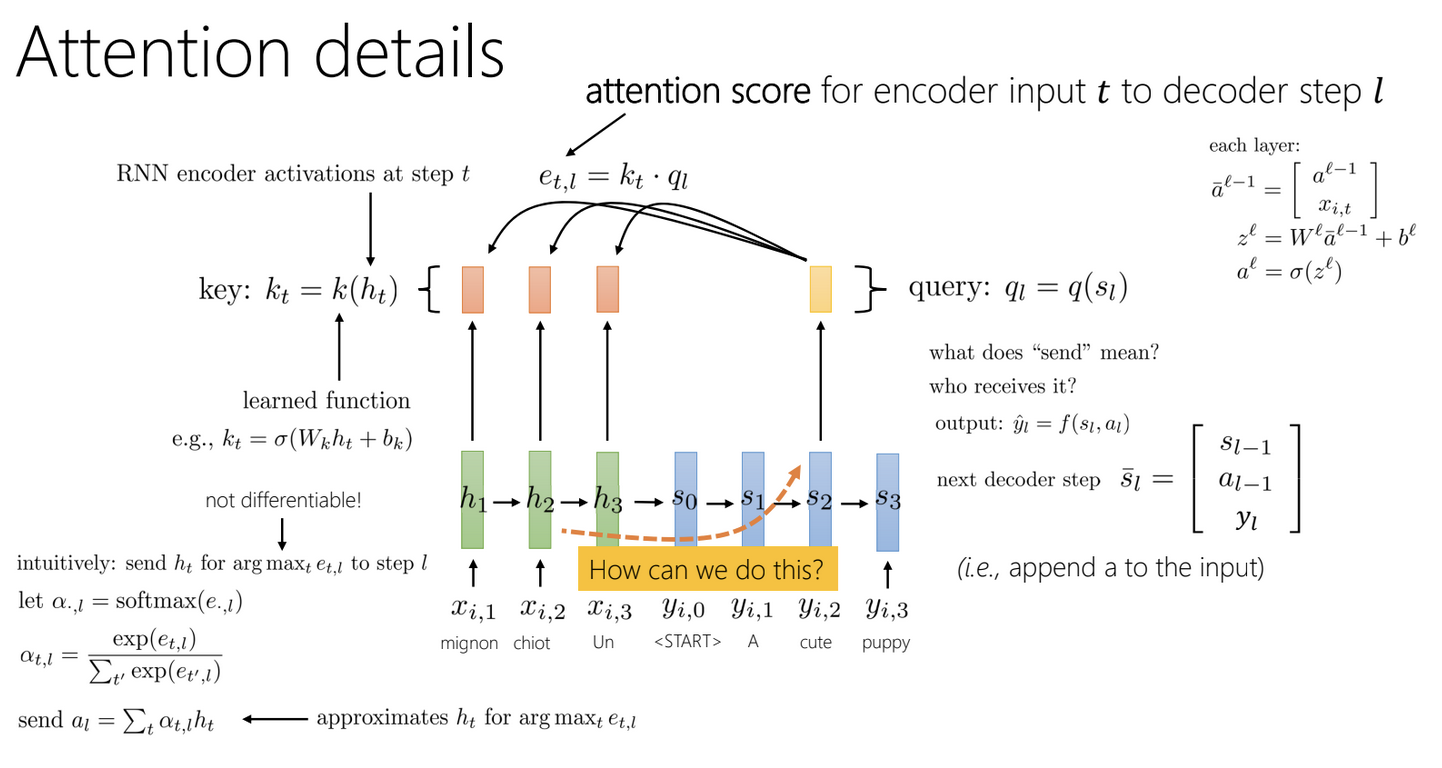
\includegraphics[scale=0.5]{images/lec11-4.png}
		\end{center}
		\begin{itemize}
			\item Suppose you're at \( s_2 \), and you're looking to query.
				To compute the keys, you take the hidden input \( h_t \) at 
				every layer, and you put it through a function \( k(h_t) \). \( k \) 
				could be as simple as the identity, but it can also be a simple 
				learned function as well (e.g. \( k_t = \sigma(W_k h_t + b_k) \)). 
			\item When you're query, you put it through a query function \( q_{l} =
				q(s_l) \). \( q_l \) is a vector representing some concept, and
				we take the inner product of \( q_l \) with every input \( k_t \).
				This quantity \( e_{t, l} \) is called the \textbf{attention score}.  
			\item Intuitively, we would like this to be a database lookup, which
				would basically be the same as looking for \( \argmax e_{t, l} \).
				But, because this is not differentiable, we normally use a softmax
				instead.  That is:
				\[
					\alpha_{t, l} = \frac{\exp(e_{t, l})}{\sum_{t'} \exp(e_{t', l})}
				\]
				Now, the combination of all of these is a normalized probability
				distribution, then we take a linear combination of the attention
				score with the information in the input sequence back. That is, we
				send \( a_l = \sum_t \alpha_{t, l} h_t \) back. Basically, this
				ensures that the things which are sent back with high probability are
				the ones that correspond highly with the data.  
			\item After sending \( a_l \) back, we can then use this information
				combined with \( s_2 \) to finally get a prediction \( \hat{y}_{2}
				\).   
			\item The number of attention scores you have depends on the length of
				the input string. The computational complexity is then dependent on
				the length of your input. 
		\end{itemize}
	\item Some general examples of \( k(t) \) and \( q(t) \) are just the identity
		function:
		\[
			k_t = h_t \quad q_l = s_l
		\]
		so the decoder is just the inner product between the encoder and decoder. You
		can also use more complicated functions, such as:
		\[
			k_t = W_k h_t \quad q_l = W_q s_l
		\]
		where \( W \) is a parameter we augment by (\question{is this learned?}). On
		the decoder side, you then have:
		\[
			e_{t, l} = h_{t}^{\top} W_k^{\top} W_q s_l = h_{t}^{\top}W_e s_l
		\]
	\item You can also do weird things with the returned \( a_l \) as well. Instead
		of just taking the dot product of the attention score with each layer, you
		can also use a learned function here, so you return
		\[
			a_l = \sum_t \alpha_t v(h_t)
		\]
		where \( v(h_t) \) is some learned function.  

		\question{We keep saying this "learned function", how do you learn functions
		like this? Do you have another neural net that does this?}
	\item Attention is a \textbf{very} powerful tool! There is no longer a bottleneck
		because each layer can just use attention. This is very similar to how
		resents work -- we're shortening the gradient path, so this makes the neural
		net better. 
\end{itemize}
\subsection{Transformers}
\begin{itemize}
	\item Is attention all we need? Do we even need the recurrence or the
		autoregressive model? The answer is no, and what we can actually do is just
		rely only on attention. This is what transformers are. 
	\item The only issue you have with the current model is that you can only look at
		the key vectors for the input pairs, but not the decoding layers. To solve
		this, we implement \textbf{self-attention}. So, we basically make a key
		vector for \textit{every layer}, including the ones in the decoding network.
	\item Refer to the following diagram:
		\begin{center}
			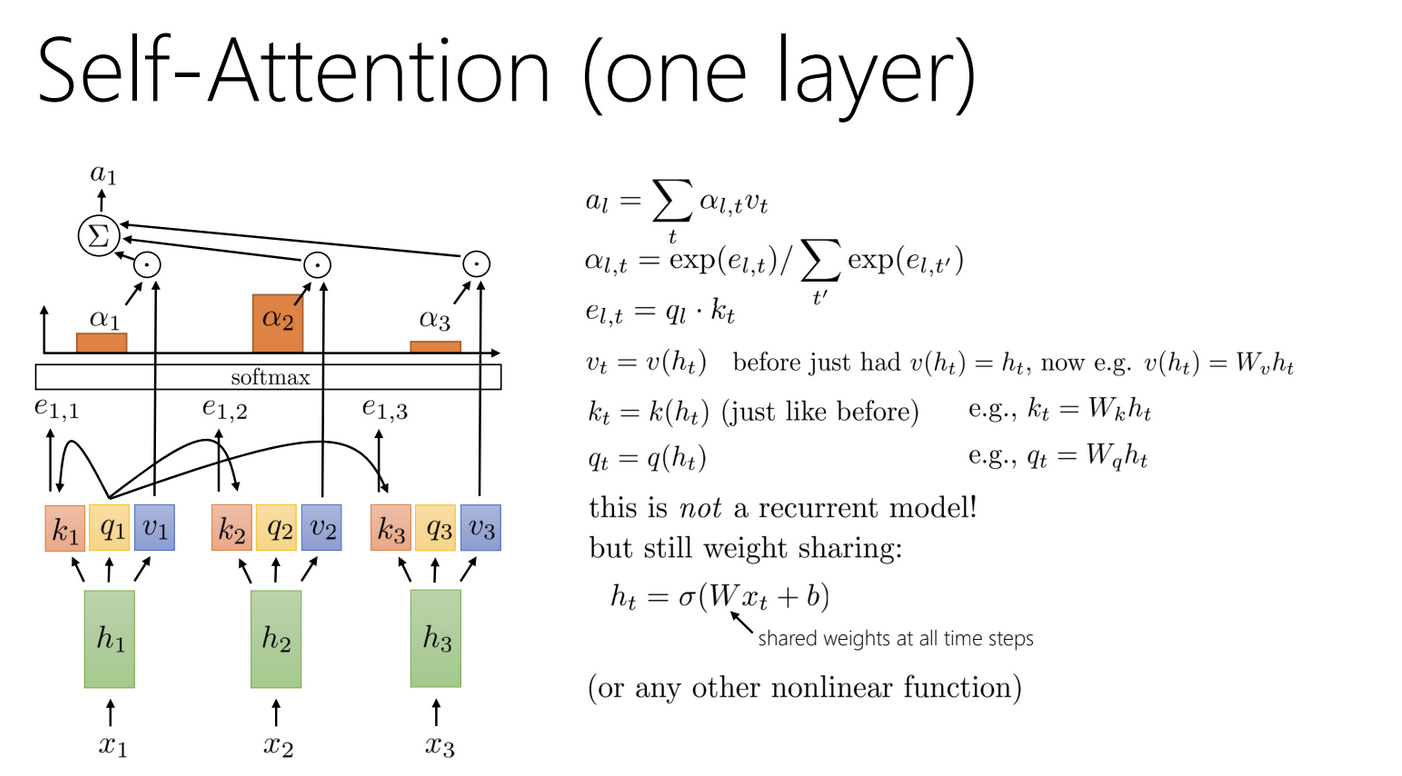
\includegraphics[scale=0.5]{images/lec11-5.png}
		\end{center}
		\begin{itemize}
			\item The intermediate arrows are now gone, and instead it's replaced by
				these \( k_i, q_i, v_i \) values. We still have a shared weight \(
				h_t = \sigma(W x_t + b) \), but they are no longer connected to each
				other. 
			\item Now, each layer has a value \( v_t \), which is defined by \(
				v(h_t) \), just as before. The key vector is also stored, in the same
				way as before \( k_t = k(h_t) \). The query is also the same as
				before. 
			\item So basically, this is a very dense version of what we had before --
				instead of having the keys in the encoder and the queries in the
				decoder, they are now all in the same system (so to speak). 
			\item If you're querying for \( h_1 \), then you query through \( k_1,
				k_2, k_3 \), and compute the attention in the same way we did before.
				The only difference is that you're querying your own key \( k_1 \) as
				well. 
			\item \( a_l \) is defined the same way, through the softmax, etc. 
		\end{itemize}
	\item Now that we've removed the recurrence, this means that the network is now
		permutation equivariant: if you switch up the order of \( h_i \) the output
		doesn't change, which is bad.  
	\item You can also stack attention layers on top of each other in the same way
		you stack a convolutional neural network. 
	\item Some issues with our model so far:
		\begin{itemize}
			\item Lack of sequence information: by removing the recurrence we've
				removed the ordering.  

				To fix this, we just force-feed position information into \( h(t) =
				f(x_t, t)\). If you just feed it in something simple (like 1, 2, 3,
				...), it actually
				doesn't do very well. What people actually do is give it a positional
				encoding \( p_t \) which is a giant vector of sines and cosines. 
			\item Multi-headed attention: in the same way you can have multiple
				kernels for your neural network, you can also have an attention layer
				for each kernel, which is called multi-headed attention.
				
				You can do multi-headed attention in parallel, the mechanisms are
				exactly the same, except in a higher dimension because we have more
				queries, keys, and values. 
			\item Linearity: each successive layer is linear in the previous one

				Fixing this just requires you to add a some nonlinear function in
				between the attention layers. 
			\item Masked decoding: How do we prevent attention lookups into the
				future?  

				This is mainly an issue caused by addressing the first issue -- when
				we bake an ordering into the system, then we have to restrict what
				each layer can query, which we can do by modifying the dot product to
				be:
				\[
					e_{l, t} = \begin{cases}
						q_l \cdot k_t & t \leq l\\
						-\infty & \text{otherwise}
					\end{cases}
				\]
				This solves the issue because now you'll get a \( -\infty \)
				attention score for the things you're not supposed to look at. 
				
				\comment{Note that throwing this into the softmax will give you \(
				e^{-\infty} = 0 \), so it does work out as expected.}
		\end{itemize}
	\item And now we've essentially built a transformer. Nowadays, transformers
		usually just refer to this stacking of self attention layers. 
	\item Some downsides is that this is pretty slow, as it runs in \( O(n^2) \),
		compared to \( O(n) \) (roughly) due to backpropagation. It's also slightly
		harder to implement. 

		That said, it also has many benefits, which outweigh the downsides: they have
		much better long-range connections, they're much easier to parallelise, and
		you can also make them much deeper than you can with RNNs.  
\end{itemize}

	\section{Dynamic Programming I}

	\subsection{Fibonacci Numbers, revisited}
	\begin{itemize}
		\item Imagine computing Fibonacci numbers; there's a lot of repeated calculations! For instance, 
			$F(1)$ is computed $2^n$ times when we're looking for $F(n)$!
		\item To optimize this, store each successive computation of $F(n)$ into an array that we access, 
			so that we only need to compute each $F(k)$ exactly once.
		\item This is called \textbf{memoization}, where we store things in a ``memo,'' to be accessed by our 
			algorithm later on. 
	\end{itemize}
	\subsection{Elements of Dynamic Programming}
	\begin{itemize}
		\item There are a couple hallmarks of DP:
			\begin{enumerate}
				\item Subproblems, or ``optimal substructure''. Refers to the fact that large problems 
					can be broken up into smaller subproblems. For Fibonacci, this means that 
					$F(n)$ is recursively expressed in terms of smaller subproblems.
				\item Overlapping subproblems: A lot of subproblems overlap with one another. We recurse to 
					smaller subproblems, and in doing so we see that a lot of computation 
					is repeated. The solution to this is to use memoization, so that 
					each computation is done only once.
		\item There are two ways to do DP:
			\begin{itemize}
				\item Top-Down: start from the largest subproblem and recurse to smaller subproblems. 
					This often involves recursion.    
				\item Bottom-up: start from the smallest subproblems then work to larger subproblems.
					Memoization still happens; we just fill the table from the small to 
					largest problems. In this method, this doesn't need a recursive call. 
			\end{itemize}
		\end{enumerate}
		\item The mathematical runtime of top-down and bottom-up are the same.
		\item The computation structure for DP actually looks awfully similar to a DAG. 
		\item If we view every subproblem as a node in the graph: construct it in such a way that 
			an edge $i \to j$ exists if the solution to subproblem $j$ directly depends on the solution to of 
			subproblem $i$. 
		\item Consider a topological sort on this DAG: then the bottom-up solution directly follows the 
			conputation of this DAG! 
			\begin{itemize}
				\item In the top-down framework, we are filling up the memo table in topological sort order, 
					since that table is still being filled from bottom up.
			\end{itemize}
	\end{itemize}
	\subsection{Shortest Paths on DAGs}
	\begin{itemize}
		\item We're given a DAG with a source $s$. We want to find the cost of the shortest path from 
			$s$ to $u$ for all $u \in V$. We also want to do this in linear time, 
			$O(n + m)$.
		\item We can always run a topological sort on this DAG in $O(n + m)$ time. Our subproblems 
			are the distances from $s$ to $u$ for every node $u$.
		\item After ordering in topological sort, we can just go down this graph \textit{in topological 
			order!} This means that the structure of the DP tree is the same as that of the topological sort.
		\item In terms of our recurrence relation, $\dist(u) = \dist(v) + \ell(u, v)$. Here, 
			$\dist(v)$ is implied to be memoized, since it's already a solved problem.
		\item This is an $O(n +m)$ solution to this problem!
	\end{itemize}
	\subsection{DP Recipe}
	\begin{enumerate}[label=\alph*)]
		\item Identify the subproblems (i.e. find the optimal substructure)
		\item Find a recursive formulation for the subproblems: just try to solve it via recursion and 
			see where it gets you.
		\item Design the DP algorithm -- fill in a table, starting with the smallest sub-problems and 
			building up. 
	\end{enumerate}
	\subsection{Shortest Paths with $k$}
	\begin{itemize}
		\item Here we consider the same problem of finding shortest path, but we're restricted to use at most 
			$k$ edges. 

			\question{Fill this out from lecture recordings}
	\end{itemize}
	\subsection{All-Pair Shortest Paths}
	\begin{itemize}
		\item Here, instead of finding the shortest path from a singular source node, we want to find 
			it for all pairs of nodes. 
		\item Input: again a graph with no negative cycles.
		\item Naively, we can run Bellman-Ford on all nodes, but this would take $O(nm)$ a total 
			of $n^2$ times, so our total runtime could be as large as $O(n^4)$ for dense graphs.
			Therefore, we're looking for a better algorithm.
		\item Identify the subproblem: subproblem $k$: for all pairs, find the shortest $u \to v$ path 
			whose internal vertices (so the path they take) only use nodes $\{1, 2, \dots, k\}$.
			\begin{itemize}
				\item In other words, there's a collection of $k$ nodes, and the path from $u \to v$ 
					\textit{only} uses these nodes.
			\end{itemize}
		\item Recursion: When we have the set from $\{1, \dots, k\}$, we want to find the relation between 
			this set and how to expand this set. There are a couple ways that the new 
			node can be added:
			\begin{itemize}
				\item Case 1: The new node added does not lie on the path: then nothing really changes, so 
					$\dist_{k +1}(u, v) = \dist_k(u, v)$.
				\item Case 2: The shortest path uses the added node: this path can be broken into two 
					parts: the shortest $u \to (k+1)$ path and then the shortest $(k+1) \to v$ path. 
					Both of these paths are already computed (by definition of them only using 
					the set $\{1, \dots, k\} $), so we just have to add these two up. 
				\item To combine these two, we find the minimum of these two to find whether the 
					path from $u$ to $v$ has changed or not.  
			\end{itemize}
		\item Runtime: Each update is $O(1)$ time, and we have to loop over $u, v$ a total of $k$ times, 
			so overall $O(n^3)$ runtime. 
		\item This is called the \textbf{Floyd-Washall Algorithm.}
	\end{itemize}

	\section{Dynamic Programming II}
	We will look more at how to choose subproblems (step 1 of our ``recipe'' to solve DP problems)
	Some problems we'll look at today:
	\begin{itemize}
		\item Longest increasing subsequence
		\item Edit distance
		\item Knapsack Problem
	\end{itemize}
	Pay attention to the information our subproblems need to be storing. 

	\subsection{Longest Increasing Subsequence}
	\begin{itemize}
		\item Given an array of integers $\left[ a_1, \dots, a_n \right]$, and we want to return the length 
			of the longest increasing subsequence of the input. (the selection of the indices \textbf{doesn't 
			have to be contiguous})
		\item We're going to deal with 1-indexed arrays here. 
		\item Why is this useful? This problem is one processing step used in a lot of other algorithms, 
			and even the game of Solitaire (also called Patience Sorting)
	\end{itemize}
	\subsubsection{Subproblems}
	\begin{itemize}
		\item Which of the following is better?
			\begin{itemize}
				\item $L[j]$ is the length of the LIS in the array $\left[ a_1, \dots, a_j \right] $ for 
					$j = 1, \dots, n$. 
				\item $L[j]$ is the length of the LIS in array $\left[ a_1, \dots, a_j \right] $ that 
					ends in $a_j$ for $j = 1, \dots, n$.

					\comment{The second one is far better, because we keep track of $a_j$ information.}
			\end{itemize}
		\item The second subproblem is better, because keeping track of $a_j$ is very valuable when we are 
			trying to recurse back in our DP problem. 

			If we don't keep track of $a_j$, we don't have any information of the last element of our 
			LIS subproblem, so we don't know how to attach it. 
		\item \textbf{Whatever the subproblem is not storing/not stating is going to be taken away from you.
			You can only observe things that the subproblem is storing/stating}
		\item To add, there are two cases:
			\begin{itemize}
				\item Suppose $a[j] \le a[i]$. Then we cannot add $a_j$ because it's not part of the 
					longest increasing subsequence. Therefore, $L[j]$ (the LIS up to $j$) is the same as 
					$L[i]$. 
				\item Otherwise, $a[j] > a[i]$, so we can add it to the LIS (so $L[j] = L[i] + 1$).
					
					\question{How is it possible that $a[j] \le a[i]$?}

					\answer{There could be an increasing sequence that grows slower that isn't counted in 
					the $i$-th iteration} 
				\item Therefore recursively, we have to apply the following:
					\begin{align*}
						L[i] &= \max_{i < j} \{L[i]: a_j > a_i\} + 1\\
						L[1] &= 1
					\end{align*}
					We want the maximum because we want the \textit{lonegest subsequence} to tack $a_j$ 
					onto.
			\end{itemize}
		\item In total, there are $O(n)$ subproblems, and each subprolbem has $O(n)$ time, so in total 
			we have an $O(n^2)$ runtime. 
	\end{itemize}

	\subsection{Edit Distance}
	\begin{itemize}
		\item Given a string $S[1, \dots, m]$ and $T[1, \dots, n]$, we want to find the smallest number of 
			edits to get us from $S$ to $T$. 
		\item Allowed operations: insert a character, delete character, change character.
		\item Why is this useful? Autocorrect, autocomplete in search engines and also DNA analysis of 
			similarities.
	\end{itemize}
	\subsubsection{Cost of Alignment} 
	\begin{itemize}
		\item Rather than thinking about distance in terms of \textit{moves}, instead we can think about 
			the cost of alignment. In other words, we look at the number of columns that don't agree.
			\begin{align*}
				&\texttt{S-NOWY} & \texttt{SN-OWY}\\
				&	\texttt{SUNN-Y} & \texttt{SUNN-Y}\\
				&\text{Alignment of cost 3} & \text{Alignment of cost 4}
			\end{align*}
	\end{itemize}
	\subsubsection{Subproblems}
	\begin{itemize}
		\item We define a 2D array to keep track of subproblems, where 
			\[
				E(i, j) = \text{EditDist}(S[1, \dots, i], T[1, \dots, j])
			\] 
			So this defines the cost of optimal alignment for strings $S[1, \dots, i]$
			into $T\left[ 1, \dots j \right] $.
		\item What are the different ways we can align the subproblems?
			\begin{itemize}
				\item $S[i]$ is dangling, $T[j]$ is dangling, $S[i]$ and $T[j]$ are both fully aligned. 
					Visually:
					\begin{center}
						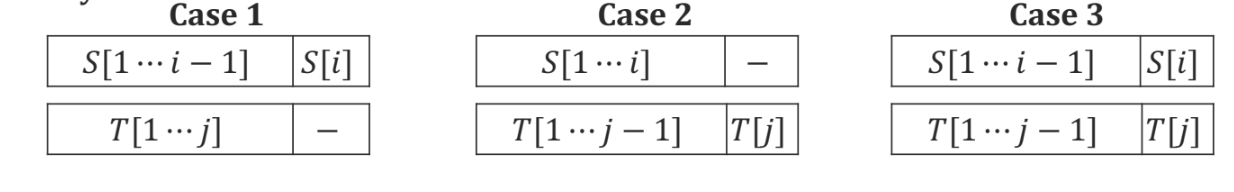
\includegraphics[scale=0.5]{alignment.png}
					\end{center}
					\comment{We add in one at a time, so there can only be one dangling letter (or none) 
					at a time!} 
			\end{itemize}
		\item We recurse based on the cases:
			\begin{itemize}
				\item Case 1: $S(i, j) = S(i-1, j) + 1$.
				\item Case 2: $S(i, j) = S(i, j-1) + 1$. 
				\item Case 3: $S(i, j) = S(i-1, j-1) + 1(S[i] \neq T[j])$.
				\item Base cases: $S(i, 0) = i$, $S(0, j) = j$. 

				The 1 represents an indicator function that counts the number of misaligned characters.
			\end{itemize}
		\item During the recursion step, we want to fill $S(i, j)$ with the \textit{minimum} value 
			of these three, since we want to minimize the number of edits. We will store this information 
			(memoizing) in a 2D array.
		\item We have to traverse our array either row by row, column by column, or diagonally. This is because
			we need to ensure that all three subproblems that we're considering have already been 
			computed. 
		\item Pseudocode:
			\begin{center}
				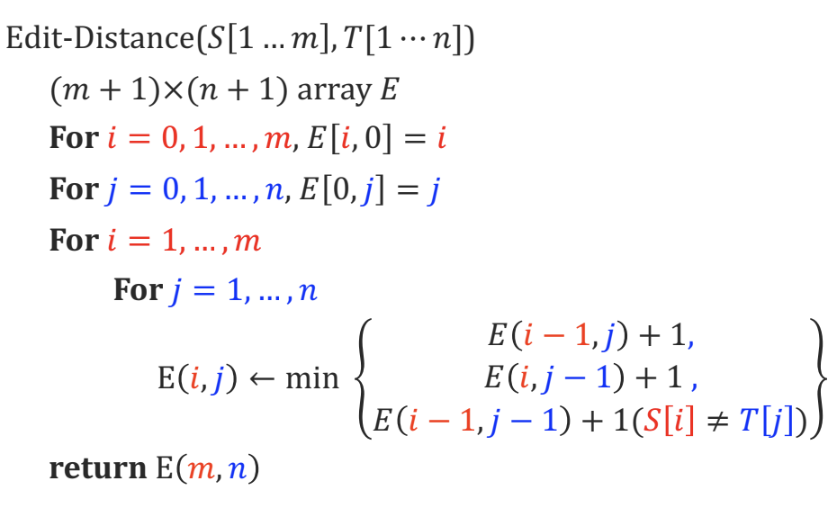
\includegraphics[scale=0.5]{alignment-pseudocode.png}
			\end{center}
		\item Runtime: there are $O(mn)$ subproblems, since we have a 2D array of dimension $mn$. At each 
			subproblem, we are only computing a minimum, which is $O(1)$ runtime, so we just have 
			$O(mn)$ runtime. 
			
			\question{Isn't the indicator also computed at this step? Why is that not accounted in the runtime?}

			\answer{The indicator is run in constant time, since we're only looking at the $i$-th character 
			in comparison to the $j$-th character.}
	\end{itemize}
	\subsection{Knapsack (with repetition)}
	\begin{itemize}
		\item A weight capacity $W$ and $n$ items with weights and values $(w_i, v_i)$. We want to output
			the most valuable collection of items whose total weight is at most $W$.
		\item We will be selecting with repetition here, but there is an easier variation where we don't
			consider repetition.
	\end{itemize}
	\subsubsection{Subproblems}
	\begin{itemize}
		\item For all $c \le W$, we want to consider the best achievable arrangement for knapsack of 
			capacity $c$. 
		\item Recurrence: For a given item $i$, then once we put it in the knapsack there are only $
			c - w_i$ capacity that remains to be optimized. This is our recurrence relation.
			\[
				K(c) = \max_{i : w_i \le c}\{v_i + K(c - w_i)\} 
			\] 
			This is a maximum over the value because we want to maximize the value being put in our 
			knapsack.
		\item We will store this information in an array of size $W + 1$, since we need a $K(0)$ element.
			\begin{center}
				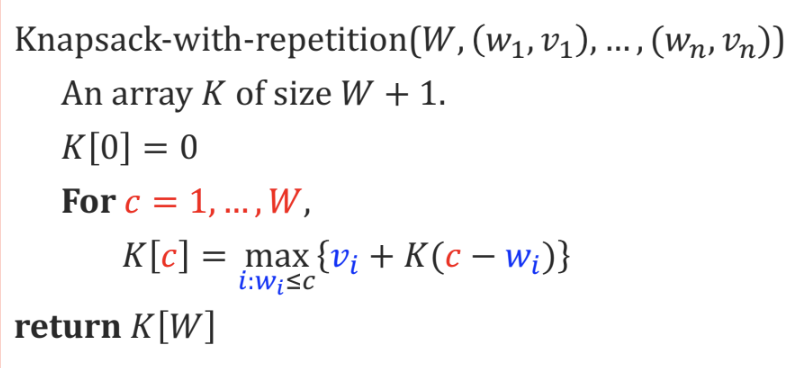
\includegraphics[scale=0.5]{knapsack-repetition.png}
			\end{center}
		\item Runtime: There are $O(W)$ subproblems, and at each subproblem, we have maximally $n$ items
			 we need to check. So in total, we have $O(nW)$ runtime.
		 \item Generally we want to think of the runtime in terms of the input. For graph problems, we looked 
			 at the input size $|V|$ and $|E|$. But for this problem, $W$ takes $\log(W)$ bits to represent 
			 $W$. So the input size is $\log(W)$. For the weights of the items themselves,
			they also only have at most $\log(W)$ bits, Therefore, the total runtime is $O(n \log W)$. 

			This kind of algorithm is polynomial in $n$, but not $W$. This is called a \underline{pseudo-
			polynomial} algorithm, since it's an algorithm that's polynomial given the numerical value 
			of the input but not in the input size.
	\end{itemize}

	\section{Dynamic Programming III}

We'll look at more examples today of DP.

\subsection{Knapsack (without repetition)}
\begin{itemize}
	\item Start with a recap with knapsack: had a weight capacity $W$, and a set of items with individual 
		weights $(w_i, v_i)$, and we wanted to look at the most valuable combination of items.
	\item Now, we're going to look at this problem with the with the constraint that \textit{we cannot 
		choose with repetition}
	\item To solve, look at how we solved the problem with repetition: introduced $K(c)$ which gets us 
		the best achieveable value for a capacity $c \le W$. The issue with trying the same thing 
		is that our subproblems don't track which items have already been used. Why not keep track of both? 
\end{itemize}

\subsubsection{Subproblems}
\begin{itemize}
	\item Introduce a 2D array: essentially solve the problem for smaller knapsacks and also smaller 
		capacities. Then expand in two directions: in terms of the number of items and also the 
		capacity.
	\item So keep track of all weights $c \le W$ and all items $j \le n$. Define $K(j, c)$ to be the 
		optimal solution to the knapsack for capacity $c$ and items $\{1, 2, \dots, j\} $. (It doesn't 
		need to use all the items from 1 to $j$.
	\item For each $K(j, c)$, we recurse smaller subproblems:

		\textit{Case 1:} The optimal solution on items 1 through $j$ doesn't use item $j$. 
					Here, $K(j, c) = K(j-1, c)$.

			\comment{Note that this is not equivalent to $K(j-1, c - w_j)$, since the $w_j$ could be 
			distributed among other items.}

		\textit{Case 2:} the optimal solution on items 1 through $j$ uses item $j$.
		Here, $K(j, c) = K(j-1, c - w_j) + v_j$. We add $v_j$ to $K$ since we're now using item $j$.   

		The intuition here is that we use the optimal solution without item $j$, then add in item $j$ 
		at the end. 
\end{itemize}
\subsubsection{Implementation}
\begin{itemize}
	\item So let's formalize this:
		\[
			K(j, c) = \max\{ K(j-1, c), v_j + K(j-1, c - w_j)\}
		.\]
		with base cases $K(0, c) = 0$ and $K(j, 0) = 0$. The base cases make sense since with no items our 
		optimal value is 0, and with no allowed weights then the optimal value is also 0. 

	\item Looking at $K(j, c)$ it only relies on the subproblmes $K(j-1, c)$, or $K(j-1, c - w_j)$, so we're 
		only looking at row $j-1$, and different elements in that row. This tells us about the order in which 
		we should be solving the subproblems: we could either do this row by row or column by column. 
	\item For runtime, ther eare $O(nW)$ subproblems, and in each subproblem we're doing constant 
		work (memory access), so therefore the total runtime is $O(nW)$, just like knapsack with repetition. 
	\item For space complexity, notice that each $K$ only depends on the previous row, so once we've 
		moved onto the 3rd row, we no longer need the first. We can delete this from memory, so the optimized 
		space complexity is $O(W)$. 
\end{itemize}
\subsection{Traveling Salesperson Problem}
\begin{itemize}
	\item A notoriously difficult problem, and DP helps us get a \textit{slightly} better runtime. 
	\item Input: Cities $1, \dots, n$ and pairwise distances $d_{ij}$ between cities $i$ and $j$. We want to 
		find a ``tour'' of minimum total distance (so we need to visit every city exactly once and 
		return to the city we started at).
	\item The naive brute-force algorithm basically is the one where we have to go through all possible 
		tours: there are \( n! \in O(n^n) \) possible tours, which makes this computation very expensive. 
	\item Dynamic programming gives us $O(n^2 2^n)$. (this is nearly optimal, beating $O(n 2^n)$ is theorized
		to be impossible)
		\begin{itemize}
			\item To give an illustration of the difference DP makes, if $n = 25$, then $O(n!) \approx 10^{25}$, 
				whereas $O(n^2 2^n) \approx 10^{10}$, so we're already better by 15 orders of magnitude. 
		\end{itemize}
\end{itemize}
\subsubsection{Subproblems}
\begin{itemize}
	\item One challenge of TSP is that subproblems aren't exactly solving the problem. If we just look at 
		TSP for a subset of our graph, that doesn't necessarily give us a solution to the larger problem, since 
		we're looking for cycles. Instead, we think of ``partial solutions'' to our graph. 
	\item We think of the subproblmes as starting from city 1, ends in city $j$, and passes thorugh all cities
		in a set $S$ (which includes city 1 and \( j \)). Visually:
		\[
			1 \to i_1 \to i_2 \to \dots \to j			
		\]
		So we want to formally define $T(S, j)$ to be the length of the shortest path visiting 
		all cities in $S$ exactly once, starting from 1 and ending at $j$. 
\end{itemize}
\subsubsection{Recurrence Relation}
\begin{itemize}
	\item How to compute $T(S, j)$ using smaller subproblems? Well, look at the string again:
		\[
			\overbrace{\underbrace{1 \to i_1 \to i_2 \to \dots \to i}_{T(S \setminus j, i)} \to j}^{T(S, j)}
		\]
		To actually talk about $T(S, j)$, then we need to add $d_{ij}$ onto every $T(S \setminus j, i)$. However,
		what is annoying is that we actually don't know which city is second to last, so we'll need 
		to consider every possible city $S \setminus j$. 
	\item So, we'll have to pick the minimum over all $i \in S$ such that $i \neq j$. Formally:
		\[
			T(S, j) = \min \{T(S \setminus j, i) + d_{ij} | i \in S \land i \neq  j\} 
		\]
	\item Our base cases are $T(\{1\} , 1) = 0$, this is fairly trivial. We also want that $T(S, 1) = \infty$.
		The reason we want this is because we're talking about incomplete paths, so $T(S, 1)$ is not 
		a valid non-cycle. Hence, we want to set it to $\infty$.  
	\item We're not done though, because we have to do something to get us back to a cycle! At the end of 
		the recursion step, we'll want to add the final edge $(j, 1)$ back, but adding only the minimum:
		\[
			T(S, 1) = \min_{j \neq  1}\{T(\{1, \dots, n\}, j) + d_{j 1}\}
		\] 
\end{itemize}
\subsubsection{Implementation}
\begin{itemize}
	\item Want an array of size $2^n \times n$, and start with base cases. Then work on the recursion:
		\begin{center}
			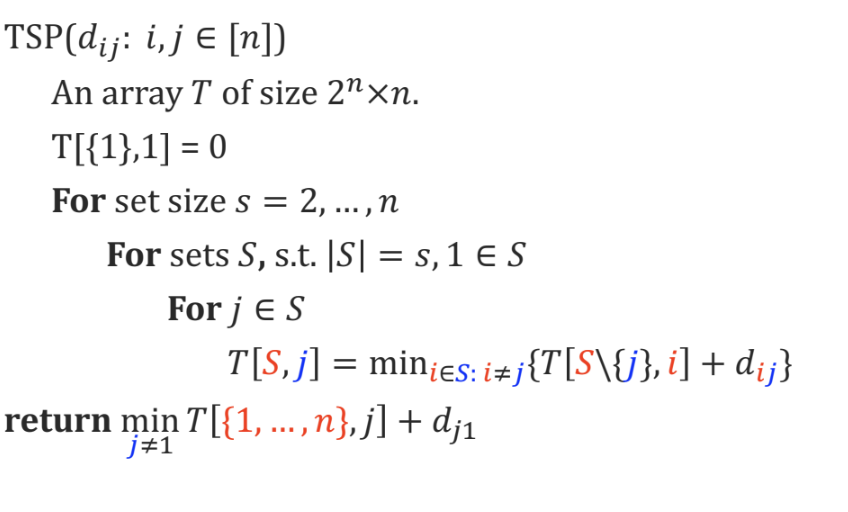
\includegraphics[scale=0.5]{TSP-code.png}
		\end{center}
	\item For runtime, there are $O(2^n \times n)$ subproblems, and on each layer we're doing $O(n)$ work, since
		we're checking the minimum across $n$ nodes every iteration. So, we have $O(n^2 2^n)$ as 
		the final runtime. 

		\question{How do we explain that \(n^2 2^n\) is the number of subproblems?}

		\answer{$O(n)$ work at every step, then $n \times 2^n$ subproblems. There are $2^n$ subsets, and in 
			each subset we can choose a $j$ to exclude, which we can upper bound by saying that there are $n$ 
		of these. So $n \times 2^n$ is a tight upper bound on the number of subproblems.}
\end{itemize}
\subsection{Independent Sets in Trees}
\begin{itemize}
	\item We're given an undirected graph \(G = (V, E)\), and want to output the largest independent 
		set of \(G\).
	\item Recall that a set \(S \subseteq V\) is considered independent if there are no 
		edges between \(u, v \in S\).
	\item This is also a notoriously hard problem, for general graphs. There isn't a polynomial time algorithm 
		that does this. But for trees, we're in luck!

		\question{Why isn't the solution just selecting every other layer?} 

		\answer{There are instances where we can pick from two consecutive layers and still not have an edge. 
		Consider the tree:
			\begin{center}
				\begin{tikzpicture}
					  \node {A}
					child {node {B}}
					child {node {C}}
					child {node {D}
					  child {node {E}}
					  child {node {F}}
					};
				\end{tikzpicture}
			\end{center}
			Our greedy algorithm would select either \(\{A, E, F\} \) or \( \{ B,C,D\} \), but the optimal set
			is actually 
		\(\{B, C, E, F\} \), so this proves that our algorithm isn't optimal.}
	\item For trees, we know that they don't have cycles, so we can pick any node and say that that is the root.
		By doing this, we can get a ``natural ordering'' of the subproblems. 
\end{itemize}

\subsubsection{Subproblems}
\begin{itemize}
	\item Let \(I(v)\) be the size of the maximum independent set in the subtree that is rooted at \(v\). 
	\item Why is this a good subproblem? Becuase it's easy to write a recursion relation for it!
	\item For the subproblems, there are two cases:

		\textit{Case 1:} \(v\) (the root of the tree) is part of the optimal independent set. This 
		means that the children aren't allowed to be part of the independent set. So if we take $v$, we can't 
		take any of the subproblems. So we need to look instead at the \textit{grandchildren} of \(v\) to join.
		Here, we'd write this as:
		\[
			I(v) = 1 + \sum_{u\  \in \text{ grandchildren}} I(u)
		\] 
		We add 1 here because we're including \(v\) now. 

		\textit{Case 2:} \( v\) is not part of the optimal independent set. Here, we would just take 
		the maximum of the children. Then:
		\[
			I(v) = \max_{u \ \in \text{ children}} \{I(u)\} 
		\] 


		So we'll take the max of these two cases:
		\[
		I(v) = \max \{1 + \sum_{u \ \in \text{ grandchildren}} I(u), \sum_{u \ \in \text{ children}} I(u)\}
		\] 
		Also, base cases is that $I(\text{leaf}) = 1$. 
\end{itemize}
\subsubsection{Implementation}
\begin{itemize}
	\item We need a data structure to store the tree easily, and also make sure that every child is processed 
		before the parents are. Well, we can iterate through the graph in post decreasing post order! 
	\item The runtime of DFS on trees is \(O(|V|)\), and each edge is looked at \(\le 2\) times -- once 
		for the children and also once for its grandchildren, so each subproblme takes constant time. 
	\item So that the total work is \(O(|E|) = O(|V|)\), since \(|E| = |V| - 1\).
\end{itemize}

	\section{Nearest Neighbor and Metric Learning}
\subsection{Parametric vs. Non-Parametric Models}
\begin{itemize}
	\item So far, we've mostly focused on parametric models, where we aim to learn \( p(y \mid x) \), through
		the use of a parameter \( \theta \):
		\[
			p_{\theta}(y \mid x) \approx p(y \mid x)
		\]
	\item The parameters are determined through MLE (or some other method), and generally the data is then
		thrown away. Today, we will look at non-parametric models (i.e. models which don't consider a
		parameter \( \theta \)). In this case, we will keep the training examples, and in effect the number
		of training parameters grows with \( n = |\mathcal{D}| \). In some sense, the dataset itself is the
		parameters. 
	\item As an aside, we should cover metric spaces first: a metric space is a set \( X \) together with a
		notion of distance \( d \) between its elements:
		\begin{enumerate}[label=\arabic*.]
			\item \( d(x, x) = 0 \).
			\item \( d(x_1, x_2) > 0 \) if \( x_1 \neq x_2 \).
			\item \( d(x_1, x_2) = d(x_2, x_1) \).
			\item Triangle inequality. 
		\end{enumerate}
		One metric we commonly see in ML is called the \textit{Mahalanobis distance}, written as:
		\[
			d_M(x_1, x_2) = \sqrt{(x_1 - x_2)^{\top} M (x_1 - x_2)}
		\]
		this collapses to the Euclidean distance when \( M = I_d \).
\end{itemize}
\subsection{KNN Classifier}
\begin{itemize}
	\item Suppose you've classified some data into two classes, and now you want to classify a new point \( x
		\). To do this, we first find the \( K \) closest (using a metric \( d \)) examples in the
		pre-existing data to inform our decision on what \( x \) should be classified as. We denote this set
		as \( N_K(x, \mathcal{D}) \). 

		\question{How is the pre-existing data generated?} 
	\item We then look at the labels \( y_i \) for the points \( N_K(x, \mathcal{D}) \), and use it to
		estimate what \( p(y \mid x)  \) should be (i.e. what label we assign it):
		\[
			p(y = c \mid x, \mathcal{D}) = \frac{1}{K}\sum_{i \in N_k(x, \mathcal{D})} I[Y_i = c]
		\]
		note that this probability sums to 1 when we sum over all \( c \), so this is actually a valid
		probability distribution. In words, this means that the probability a point \( y \) is assigned a
		label \( c \) is given by the proportion of the nearest \( K \) points that are assigned \( c \).
	\item The \( k = 1 \) case is special - the partition that you get is called a \textit{Voronoi
		tessellation}. In this case, if you scatter some points onto the plane, then this division will
		partition the space up strictly based on distance and all the boundaries are just straight edges
		between classes.  

		In this special case, the classification of a new point is given by the nearest neighbor, so this is
		why you get such a special pattern.

		\question{How do you tell the classifier how many classes you should make?} 

		\answer{This is probably something you decide ahead of time; there's probably no way for you to
		"train" a model to know how many you should make.}
	\item Visually, you can also compare different \( K \) and \( K' \) nearest neighbor algorithms, and
		there is a distinction between them. For larger \( K \), the general trend is that the boundary
		between classes gets finer and not as jagged, as is typically seen in a smaller \( K \).  
	\item There is also an optimal \( K \) for classification. If \( K \) is too large, then you risk
		comparing against points that are not near your target point \( y \), and therefore you will get a
		bad classification from it. 

		This is also a general trend we observe in model training: as the model complexity increases, the
		training error decreases monotonically, but the test error reaches an optimum somewhere in between.
		This is because there are two regimes on the extremes: extreme simplicity on one end, and overfitting
		on the other. 
\end{itemize}

\subsection{KNN Generative Classifier}
\begin{itemize}
	\item Now we move to the \( K \)-nearest neighbors except this time we have a generative classifier. In
		this case, we essentially define a "ball" around each point \( x \) until we encounter \( K \)
		points, and the classification is then given by the proportion of points in that ball \( V_K(x) \)
		that are classified as class \( c \).      
	\item If you have a \textit{lot} of data, it has been shown that the KNN test error can never be worse
		than twice the optimal Bayes classifier. This is interesting to note, because the Bayes classifier
		requires \textit{much} more information about your data (the class conditionals, distribution, etc.),
		but KNN knows nearly nothing.  
	\item This is a quick aside, but basically the idea is that the space you need to check increases
		exponentially with dimension. Because the volume grows exponentially large, it becomes increasingly
		more impractical to search such a space, and so this makes KNN much worse in higher dimensions.  

		If you want to get \( \epsilon \) close to a target, by increasing the dimension you can only get 
		\( O(n^{ - 1 / d}) \) closer to the target by increasing the dimension. 
\end{itemize}

\subsection{Pros and Cons of KNN}
\begin{itemize}
	\item Pros:
		\begin{itemize}
			\item Fast, no training required.
			\item Learns complex classification functions easily, because it requires no priors.
		\end{itemize}
	\item Cons:
		\begin{itemize}
			\item High storage cost
			\item Slow at computing inference (actually performing the classification)  
			\item Very bad dimensionality scaling. 
		\end{itemize}
\end{itemize}

\subsection{Manifold Hypothesis}
\begin{itemize}
	\item The manifold hypothesis basically states that "true" high dimensional data that we care about, like
		images, videos, etc. lie in a lower dimensional manifold which is embedded in a higher dimensional
		space.   
	\item The idea then is that we essentially "embed" the data onto a lower dimensional space using a neural
		network, learn the
		space using a Euclidean metric, then you can classify using this Euclidean metric. 

		\question{Is this the approach that t-SNE uses?}
	\item The challenge then becomes: how do you define an embedding that does exactly what you want?
		Ideally, you want an embedding that pulls similar objects close to each other and pushes dissimilar
		ones apart.
	\item One of the earliest approaches to doing this was based on \textit{contrastive loss}. Basically,
		define a loss function over two points \( i, j \):
		\[
			\mathcal{L}_{ij}(\theta; m) = \mathbb I (y_i = y_j)d(z_{\theta}(x_i), z_{\theta}(x_j))^2
			+ \mathbb I (y_i \neq y_j) \max(0, m - d(z_{\theta}(x_i), z_{\theta}(x_j))^2)
		\]
		(recall that \( z(x) \) is your embedding function). 
		Essentially, you minimize the loss between similar points, while also defining a "maximum acceptable
		distance" between two dissimilar points. You require this \( m \) because otherwise, your model will
		want to push dissimilar points increasingly farther away off to infinity.  

		Tested this on the MNIST dataset and bringing this down to a 2-dimensions from 784 dimensions, and
		the results look very good.    
	\item The problem with this approach is that the "pull" and "push" terms don't talk to each other, or in
		other words this is a very binary way to approach this embedding approach. 
	\item This leads to the second approach: triplet loss. Here, the loss is given by:
		\[
			\mathcal{L}_i(\theta; m) = \max(d(z_\theta(x_i), z_{\theta}(x_i^{+}))^2 - d(z_{\theta}(x_i),
			z_{\theta}(x_i^{-}))^2 + m, 0)
		\]
		In essence this does the exact same thing: you want the first term to decrease while simultaneously
		wanting the second term to increase, but this is a more clever approach because the terms are
		combined together. 
		
		Here, \( z^{+} \) is a positive (similar) example, and \( z^{-} \) is a dissimilar (negative)
		example.  

		\question{what is the positive and negative example referring to?} 

		\answer{these are \textit{anchors} in the data, and are given as true points in the dataset.}  
	\item One issue with the triplet loss is that because there are a lot of negative examples to compare to,
		you naturally need to perform that computation many many times to get the loss for a single point.
		This leads to the \( N \)-pair loss, which lets you take a batch of negaitve samples at a time:
		\[
			\mathcal{L}(\theta; x, x^{+}, \{x_k^{-}\}_{k = 1}^{N}) = \log\left( 1 + \sum_{k = 1}^{N -
			1}\exp\left( \hat{z}_\theta(x)^{\top} \hat{z}_\theta(x_k^{-}) - \hat{z}_\theta(x)^{\top}
			\hat{z}_\theta (x^{+}) \right) \right)
		\]
		what this means is that you take a set of predefined dissimilar examples \( \{x_k\} \) and use that
		as the "push" term. 

		\question{How does this algorithm work in practice? Would you have to define a set of similar and
		dissimilar classes for every class you're working with?} 

		\comment{The reason you don't need a max function here is because \( \hat{z}_\theta(x) \) is a
			projection that only projects into a volume of a unit sphere, so there is a predefined limit to
			how far apart dissimilar points can be apart. You can also convert this interpretation into an
		equivalent one using softmax.}   
	\item There's also the world of joint embeddings: where text and images are encoded together and embedded
		onto a space: OpenAI's CLIP model was trained on an \( N \)-pair loss in a jointly embedded space.  
\end{itemize}

	\section{Network Flow}
\begin{itemize}
	\item Recently declassified (1999) document about the USSR's shipment capacity from east to west. This 
		was crucial information at the time since had a war broke out, the US could identify which 
		supply routes they could bomb.
	\item They devised a greedy algorithm called ``flooding,'' but this algorithm wasn't really optimal. It 
		was finally solved by Ford and Fulkersson, and is now called the Ford-Fulkersson algorithm.
	\item Given a directed graph $G = (V, E)$, one source vertex $s$ and a sink $t$, and for each edge $e \in E$,
		we're given a capacity $c_e$ which are integers. 
	\item We want to find the maximum amount of water from $s \to t$.  
	\item \textit{Definition:} A flow assigns a number $f_e$ to each directed edge $e \in E$ such that:
		\begin{itemize}
			\item nonnegativity: \(f_e \ge  0\) 
			\item capacity: \(f_e \le c_e\)
			\item flow in and flow out are equal: \(\sum_{u \to v} f_{u, v} = \sum_{v \to w} f_{v, w} \)
		\end{itemize}
	\item Let's also define the size of the flow $f$ to be the total quantity set from $s$ to $t$. Using 
		this definition, then the maximum flow is the one that maximizes $\size(f)$. This can be solved 
		using linear programming!
\end{itemize}

\subsection{Greedy (suboptimal) algorithm}
\begin{itemize}
	\item We'll find a path $P$ from $s$ to $t$, and send flow until it's saturated. We'll do 
		this as much as we can. We repeat this until we run out of paths.
	\item This algorithm fails on some graphs, because it uses edge $A \to B$ when that edge is suboptimal! 
		Consider the graph:
		\begin{center}
			\begin{tikzpicture}[scale=2]
				\node (s) at (0, 0) {$s$};
				\node (a) at (1, 0.7) {$A$};
				\node (b) at (1, -0.7) {$B$};
				\node (t) at (2, 0) {$t$};
				\graph[edge label = 1]{(s) ->(a) -> (t), (s) -> (b) -> (t), (a) -> (b)};
			\end{tikzpicture}
		\end{center}
		Our algorithm just looks at flow rate, so a possible path to take is $s \to A \to B \to t$, but this 
		is clearly suboptimal! Instead, we should be going from $s \to A \to t$ and $s \to B \to t$. 
\end{itemize}

\subsection{Greedy Fix}
\begin{itemize}
	\item We instead consider a residual graph, where we subtract the flow given by greedy 
		($s \to A \to B \to t$), and also generate a back edge that travels in the reverse order of the flow 
		given by greedy, so that we can backtrack if needed. 
	\item Formally, given a graph $G$ and a flow $f$ on $G$, the residual raph $G_f$ is defined as:
		For all edges \((u, v)\), if $f$ goes from $u \to v$, then the residual graph will flow from $v \to u$ 
		and the edge will have capacity $c_{u, v} - f_{u, v}$. 

		By doing this, we allow our graph to backtrack along our suboptimal path if needed.  
	\item This is the approach that Ford Fulkerson uses to find the optimal flow.
\end{itemize}

\subsection{Ford-Fulkerson Algorithm}
\begin{itemize}
	\item Find a path $P$ from $s$ to $t$ in the residual graph which is not yet saturated, and send more 
		flow along $P$. We keep repeating this until everything's saturated, and this happens 
		when all edges along one particular cut is zero. 
	\item To show that this algorithm terminates, lets' first define an $s-t$ cut is a partition of the graph
		into two sets of vertices \(L\) and \( R\) such that 
		\(s \in L\) and \(t \in R\). We define the capacity of this cut to be the sum of all capacities from 
		the edges that cross from $L$ to $R$.  
	\item Therefore, for any flow $f$ and any cut \((L, R)\), then \(\size(f) \le \capacity(L, R)\). Then, the
		flow is actually upper bounded by the minimum cut along this graph (this is our ``bottleneck'' introduced
		at the outset)
	\item Then, this means that the max flow is also given by the minimum cut, and we can show that 
		Ford-Fulkerson outputs a maximum flow by considering this relation between the flow and a cut. The proof 
		of this is outlined in lecture. 

		\question{Review the proof for this later}
\end{itemize}

\subsection{Runtime}
\begin{itemize}
	\item The number of augmenting paths must be less than $U$, where $U$ denotes the maximum flow, so 
		the update is less than $O(m + n) \cdot U$. 
	\item But what this means   
	\item There are other algorithms out there that optimizes this a little more: Edmonds-Karp gives 
		us a runtime of $O(n m^2)$, which is much better than what we have. 
	\item The best runtime was discovered last year, where we have $O(m^{1 + o(1)} \cdot \log U)$
\end{itemize}

	\section{Laplace Transform}
\begin{itemize}
	\item Laplace transforms concern the equation:
		\[:tabn
		X(s) = \int_{-\infty}^{\infty} x(t) e^{-st} \diff t
		\] 
		The basic idea is that instead of solving for \( x(t) \), we solve instead for \( X(s) \), which is 
		much easier to do sometimes than \( x(t) \). 
	\item Suppose you have an LTI system with impulse response \( h(t) \), and we input a harmonic 
		exponential \( e^{j 2\pi ft} \), then we get an output \( y(t) = H(f) e^{j 2 \pi ft}
		= H(\omega) e^{j \omega t}\). (this is the 
		eigenfunction property.)
	\item What about an input \( e^{st} \)? Then, we can express this as a convolution, which 
		happens to be written as: \( y(t) = H(s) e^{st} \), where  \( H(s) \) is the Laplace transform of 
		\( h(t) \). 
	\item Consider an input \( x(t) = e^{st} \), and since \( s \in \C \), then we can write 
		\( s = \sigma + j \omega \). Then we convolve:
		\[
		y(t) = \int_{-\infty}^{\infty} h(t) e^{s(t - \tau)}\diff \tau = \int_{-\infty}^{\infty} 
		h(t) e^{st} e^{-s \tau}\diff \tau = e^{st}\underbrace{\int_{-\infty}^{\infty} h(\tau) e^{-s \tau}\diff \tau}
		_{H(s)}
		\] 
		where the integral we defined earlier as the Laplace transform \( H(s) \). Here, we call it 
		specifically the bilateral Laplace transform of \( h(t) \). This distinction just has to do with the 
		integration bounds; a unilateral Laplace transform is defined as 
		\[
		H_{\text{uni}}(s) = \int_{0}^{\infty} h(\tau)e^{-s \tau}\diff \tau 
		\] 
		but we will normally consider bilateral Laplace transforms in this class.  
	\item Note also that the Laplace transform is also the more general case of the Fourier transform: the Fourier
		transform occurs when \( \Re(s) = 0 \). 
\end{itemize}
\subsection{Notation, Terms}
\begin{itemize}
	\item With Laplace transforms, we say that they transform between the time domain and the \( s \)-domain, and 
		it's written as:
		\[
		\mathcal L \{x(t)\}  = X(s) = \int_{-\infty}^{\infty} x(t) e^{-st}\diff t 
		\] 
		Because \( s \) is a complex number, the Laplace transform takes our 1-dimensional signal 
		\( x(t) \) and turns it into a two-dimensional signal in  \( s\)-space. 
%		\begin{center}
%			\begin{tikzpicture}
%				\draw (-3, 0) -- node[right] {\( t \) } (3, 0);
%			\end{tikzpicture}
%			\( \rightarrow \) 
%			\begin{tikzpicture}
%				\draw(-3, 0) -- (3, 0) node[right] {Real};
%				\draw (0, -3) -- (0, 3) node[left] {Imaginary};
%				\draw[red] (0, 0) -- node[right] {\( X(s) \) } (1, 2);
%			\end{tikzpicture}
%		\end{center}
\end{itemize}
\subsection{Laplace Transform Pairs}
\begin{itemize}
	\item Given a signal \( x(t) = \delta(t) \), then the Laplace transform \( X(s) = 1 \). This is seen easily 
		from the integral itself:
		\[
		X(s) = \int_{-\infty}^{\infty} \delta(t) e^{- st}\diff t = 1 
		\] 
		As a 2D diagram, we can imagine that over the entire complex plane, \( X(s) \) takes on a value 
		of 1. 
	\item Given a unit step function \( x(t) = u(t) \), then the Laplace transform \( X(s) = \frac{1}{s} \). 
		Again, just do the integral:
		\[
		X(s) = \int_{-\infty}^{\infty} u(t) e^{-st}\diff t = \int_{0}^{\infty} e^{-st}\diff t = \frac{1}{s} 
		\] 
		Note that this only works if \( \Re(s) > 0 \), otherwise we have an unbounded integral. This condition 
		is also called the \textit{region of convergence} for the integral. This actually means that 
		the Laplace transform may not be defined for all values of \( s \)!

		\comment{Note that \( \Im(s) \) doesn't matter here, since all it does is give us an overall phase 
		factor of \( e^{j \omega t} \) that has magnitude 1 all the time.}
	\item Let \( x(t) = e^{-at}u(t) \). Then, let's look at its Laplace transform:
		\[
		X(s) = \int_{-\infty}^{\infty} e^{-at}u(t) e^{-st}\diff t = 
		\int_{0}^{\infty} e^{-(a + s)t}\diff t  = \frac{1}{a + s}
		\] 
		which again, only holds true when \( \Re(a +s) > 0 \). Since \( a \) is real, then the condition 
		simplifies to \( \Re(s) > -a \), so this is our region of convergence.  
		
		\comment{We could be a little more specific with the integration:
			\[
			X(s) = \int_{0}^{\infty} e^{-(a + \sigma)t} e^{- j \omega t} \diff t = \frac{1}{j \omega ( + a + \sigma)}
			 = \frac{1}{s + a}
			\] 
			but this simplifies in the same way.  
		}

		\question{If we didn't have the \( u(t) \), then would the integral still converge?}
	\item Now consider \( x(t) = -e^{-at}u(-t) \). This is just the time-flipped version of the previous signal. 
		Visually, for different values of \( a \), this is what it looks like:
		\begin{center}
			\begin{tikzpicture}[scale=0.2]
				\draw (-10, 0) -- (10, 0);
				\draw (0, -10) -- (0, 10);
				\draw[thick, color=red, domain=0:-2]  plot (\x, {-exp(-\x)}) node[left] {\( a > 0 \) };
				\draw[thick, color=blue, domain=0:-8] plot (\x, {-exp(\x)}) node[above left] {\( a < 0 \) };
			\end{tikzpicture}
		\end{center}
		Doing the Laplace transform:
		\[
		X(s) = -\int_{-\infty}^{\infty} e^{-at}u(-t)e^{-st}\diff t  = \int_{-\infty}^{0} e^{-(a + s)t}\diff t
		= \frac{1}{a + s}
		\] 
		As before, this only holds when \( \Re(a + s) > 0 \). 

		\question{Mathematica gives \( -\frac{1}{a + s} \), why?}
\end{itemize}
\subsection{Why Laplace Transform?}
\begin{itemize}
	\item Laplace transform has many of the same properties as the Fourier transform, and due to its 
		wider scaope (i.e. having \( X(s) \) be a two-dimensional function), it allows us to take the transform of 
		functions that the Fourier transform cannot handle. 
	\item It's also useful for integral differential equations. Consider the following circuit:
		% tikz here
		The voltage readout is given by:
		\[
		Ri(t) + \left[ \frac{1}{\mathcal L }\int_{0^{-}}^{t} i(t') \diff t' + v_c(0^{-})  \right] 
		\] 
		we will see later on how the Laplace transform simplifies the calculation of this integral.  
\end{itemize}

\subsection{Region of Convergence}
\begin{itemize}
	\item The Laplace transform is also related to the Fourier transform, by a multiplication of a 
		decaying exponential:
		\[
		\mathcal L \{x(t)\}  = \mathcal F \{x(t) e^{-\sigma t}\} 
		\] 
		This also tells us why the Laplace transform is more general -- by multiplying by an 
		\( e^{-\sigma t} \), we can actually modify what \( x(t) \) is. This gives us more control, and makes 
		it a more powerful tool. 
		
		The region of convergence is defined as the set of \( s \in \C \) suhc that 
		\( x(t) e^{-st} \) has a Fourier transform. Mathematically:
		\[
		\mathcal L \{x(t) \}  = \int_{-\infty}^{\infty} x(t) e^{-at} e^{- j \omega t}\diff t  < \infty
		\] 
		We've already talked a lot about the region of convergence in the previous section, so just refer to that 
		instead. 
	\item Consider the signal \( x(t) = 3d^{-2t}u(t) - 2e^{-t}u(t) \). What is its region of convergence? Since the 
		Laplace transform is linear, we can basically just find the region of convergence for both these 
		terms, and find the common ROC to get the ROC for \( X(s) \). Doing so, we get:
		\[
		X(s) = \frac{3}{s + 2} - \frac{2}{s + 1} = \frac{s - 1}{(s + 2)(s + 1)}
		\] 
		Therefore, the region of convergence is \( \Re(s) > -1 \). 
\end{itemize}

\subsection{Properties of Laplace Transform}
\begin{itemize}
	\item These are very similar to the Fourier transform properties. We will denote the relationships 
		as \( x(t) \overset{\mathcal L}{\leftrightarrow} X(s) \). 
	\item \textbf{Linearity:} Given  \( ax_1(t) + bx_2(t) \), then the Laplace transform gives \( aX_1(s) + bX_2(s) \).
		The region of convergence contains \( R_1 \cap R_2 \), but it can be larger. For example, if you take 
		a signal with some limited ROC and consider  \( x_1(t) - x_1(t) \), then the ROC would now turn into the 
		entire plane!
	\item \textbf{Time shift:} Given \( x(t - t_0) \), then we have \( e^{-st_0}X(s) \). Very similar to 
		the Fourier transform! The proof is relatively easy, just do a change of variables. 
	\item \textbf{S-domain shift:} Given \( e^{s_0 t} x(t) \), then this gives  \( X(s - s_0) \). Again, just 
		do the integral via a change of variables. The ROC will be shifted by \( \Re(s_0) \). 

		More formally, if we let \( s' = s - s_0 \) and it has a ROC of \( R \), then the ROC of \( s \) is 
		going to be \( R + \Re(s_0) \). 
	\item \textbf{Time scaling:} For a signal \( x(at) \), then the Laplace transform gives  \( \frac{1}{a}X(s) \).
		So if we shrink in time domain, then we expand in the \( s \)-domain, just like the Fourier transform.
		The new ROC is now \( a \cdot R \). As for the proof:
		\begin{align*}
			\int_{-\infty}^{\infty} x(at) e^{-st} \diff t  &=  \int_{-\infty}^{\infty} x(\tau) 
			e^{-s \tau / a} \frac{1}{a} \diff \tau \\
			&= \frac{1}{|a|}\int_{-\infty}^{\infty} x(\tau) e^{-s \tau / a} \diff \tau = \frac{1}{|a|}
			X\left( \frac{s}{a} \right) 
		\end{align*}
		\question{study this proof later.}
		
		There is also the case where \( a = -1 \), in which case we have \( x(-t) \overset{\mathcal L}
		{\leftrightarrow} X(-s)\). 
	\item Given a signal \( \cos(\omega_0 t) u(t) \), then we get \( X(s) = \frac{s}{s^2 + \omega_0^2} \). The strategy
		is basically the same thing as the Fourier transform, where we split the cosine into 
		complex exponential form. The region of convergence is \( \Re(s) > 0 \).

		For \( \cos(- \omega_0 t) u(-t) \), then we have \( X(s) = -\frac{s}{s^2 + \omega_0^2} \). 

		\question{check this.}
	\item \textbf{Conjugation:} Suppose we have \( x(t) \) and take the complex conjugate \( x^{*}(t) \), 
		then just like the Fourier transform where \( x^{*}(t) \) corresponds to \( X^{*}(-\omega) \), here 
		we it gives us \( X^{*}(s^{*}) \).  

		This doesn't change the ROC, since the ROC only depends on the real component. 

		\question{Isn't this different from the Fourier property, where the input is not conjugated?} 

		\answer{Because the Fourier transform deals with a purely imaginary \( s \), then swapping to a negative 
		is the same as conjugating a general complex value \( s \in \C \).}
	\item \textbf{Convolution Theorem:} We have \( x_1(t) * x_2(t)  \) transforms as \( X_1(s) X_2(s) \). The region
		of convergence here is \( R_1 \cap R_2 \), since we need a place where the Laplace transform 
		always exists. 

		The mathematical steps to prove this are nearly identitcal to what we had for the Fourier transform.
	\item \textbf{Differentiation:} The derivative \( \dv{x(t)}{t} \) transforms as \( s X(s) \). This makes 
		solving differential equations to be much more approachable. The ROC will contain \( R \), but 
		can sometimes include more than just \( R \). An example where \( R \) increases 
		is the signal \( x(t) = \sin(\omega_0 t) u(t) \). 

		We know that \( x(t) \) transforms to \( X(s) = \frac{\omega_0}{s^2 + \omega_0^2} \), then 
		\( \dv{x(t)}{t}  \) will transform as \( \frac{\omega_0s}{s^2 + \omega_0^2} \). 
	\item \textbf{Differentiation in s-domain:} The function \( -t x(t) \) transforms as 
		\( \dv{X(s)}{s} \), and the region of convergence does not change. In general, for a 
		signal \( t^n e^{-at} u(t)\), this will transform as 
		\[
		X(s) = \frac{(-1)^{n} n!}{(s + a)^{n}}
		\] 
\end{itemize}






\end{document}

